\documentclass[a4paper,10pt,titlepage]{article}
\usepackage{graphicx}
\usepackage{float}
\usepackage[english]{babel}

\begin{document}
	\tableofcontents
	
	\newpage
	\section{Preface}
		This project and report is made by Jakob Bang Helvind, Kasra Tahmasebi Shahrebabak, Mark Thorhauge, Filip Hjermind Jensen, Lars Yndal Soerensen og
		Anders Brorup Joergensen. It was written for the course ’First-Year Project’ on the bachelor ”Software Development” in the Spring of 2012 at the
		IT-University of Denmark. The report is written in terms, that we believe fellow students possesses and will understand. We hope that this 
		report will give insight in the workprocess as well as the product and that all readers will enjoy reading it.
		
	\newpage
	\section{Background and Data}
	
		For this project we have been given the task of designing and creating a java-written program 
		for the exam in the course 'First-Year-Project' on 2nd semester in the bachelorprogram. The basic idea of the 
		program is, that it should use some existing mapdata of Denmark to visualize a map of Denmark and let the user search for and see a route. 
		\\This dataset is from the danish mapprovider Krak.dk and it consists of two text files. A file with all the points 
		and a file with all connections between those points.  
		\\The application should meet the following requirements:
		\begin{itemize}
		\item Draw all roads in the dataset
		\item The map-visualization should adjust acordingly to changes of the windows size
		\item The user should be able to navigate in the visualization
		\item The application should have a minimum of clutter and therefore be able to set a priority of the roads
		\item Be able to compute and show the shortest path between two points given by the user
		\item The application should have a logical, consistent and reasonable fast and responsive user interface\\
		\end{itemize}
		
		In other words, a user should be able to see a map of Denmark with a selective amount of major roads, then explore this map by zooming in and out and navigating around. A user should also be able to select two adresses, and get the shortest route between these two points calculated and shown on the map, with the map cut out to a fitting view of the route.
		 
	\newpage
	\section{Limitations}
		
		There are certain limitations that we have taken to simplify the development process and make the goal more reachable. When judging performance, memory usage, usability or other factors, we do not consider other map data than the dataset given (or a modified version), but we do develop the program in a way, so other map data can be used. We do not optimize the program for a certain browser, nor do we secure that the client can be run on all leading browsers. We develop the client user interface, but we do not develop the server user interface because it does not involve any design choices that are interesting from a learning perspective.


	\section{Problemanalysis}
		\subsection{Requirements}
To get an understanding of the requirements stated in the previous section, we will walk through these, and try to analysis what is needed to meet them, and what the different solutions could be. But first, we will list our three points of focus and use these as arguments for which solution to chose in the following analysis.\\
We want to make a program that is simple and easy to use. This means focusing on making the basics work well, and not try to implement unnecessary features and functionality.\\

Our next priority is speed over space. We want our program to perform fast, and if we can do that by using some extra     memory or heap-space, that will be the cost.\\

The last priority of ours is more code minded, and is about designing a program that is easy to extend. Maybe with new functionality, or maybe changing one of the data structures, the user interface or the platform\\
\\

Let us now focus on the requirements that we have been given. The first one is about drawing all roads in the dataset. This is one of the more abstract requirements, as there are quite a lot of possibilities on how to solve this. But it does set the framework for what we need to work on. We need to be able to read the dataset probably, and store the data structured and efficiently, so it is easy to access and use for the visualization of the roads. This structure needs to be able to pull out big portions of the dataset quite fast. Because we are going to use map data that uses coordinates, it would be obvious to use this in the data structure.\\

We need to settle on a way to show the roads graphically. There have been some guidelines for us to either use a solution programmed completely in Java, or write something for visualizing the map in a web-browser. The Java-solution is more uniform, and would be somewhat easier, as you don't need to worry about the communication between multiple programming languages. This would allow us to focus on implementing extra features, and polishing the program. With a web solution, we would cut of the graphical part of the program, and let the browser handle it. This would force some task on us, like connection and getting the encoding between the browser-client and the java-server right. But it also speaks to some of our own priorities. It will push the heavy data processing to the server. If this was a server for a web-application, space wouldn't be a big problem, and you could optimize towards speed and making the client quicker. We have chosen to go a with a browser solution\\

To visualize the map in Java, we would use the Swing-libraries. In the browser we could use different solutions. With the new HTML-5 standards, the “canvas”-element in javascript, could be used for the task. This would integrate well with the other features we would implement with javascript. The other possible solution is SVG, Scalable Vector Graphics. These would easily help us with the requirement that our program should scale when resizing the window. We will use SVG, because it is somewhat simpler, and goes well with XML, which we will use to send the map data from the server to the browser. This choice will help us with navigating around the visualization.\\

Navigating the visualization can mean many things. The basic would be moving on the three main axes, up and down, left and right, zooming in and zooming out. More features could include dragging the map around using the mouse or rotating the map. The user should feel that this is done smooth. This could be done by not loading new map data every time the user moves around the map, but keeping a buffer of loaded map around the part shown. In SVG this can be done with the “viewbox”-attribute. Then we can move this box around by changing its coordinates, and loading in more of the map, when it gets too close to the edge of the buffered zone. You don’t need new data to zoom in SVG, because it consists of vectors.\\

We eventually need to load in new map data when we zoom, because of the requirement for our program to only show the most prioritized roads. Here we have some different possibilities. We can simply determine at which level of zoom each type of road (highway, paths ect) is shown, or decide how many roads we want to see at any given time, and only take the highest prioritized of these. The problem with the first solution is that some areas are not very cluttered with roads, and would therefore look empty at a high zoom level. The other solution could have a problem with cutting roads in half, if it is not implemented a bit more dynamically. If you combine the best of the two solutions, so that you only show a decided amount of roads, but also keep in mind that you need to show all roads of the same type, you should be able to avoid most of the trouble.\\

We also need to be able to find the shortest path between points. If this needs to be done quickly, we could do it with a graph data structure, and build a Shortest Path Tree with it, from the first point until we find the second. The problem with this is that it is a different data structure that the one we use for the visualization. But if we argue that this is a web-server, and we prioritize speed over space, this would be the best choice, to have two separate data structures. We then need to build the SPT. There are multiple algorithms for doing this, we looked at the Bellman-Ford-algorithm and Dijkstra's.\\

The last requirement we were given was about making the user interface logical, consistent and reasonably fast. This fit well with our own priorities, and some of the choices connected to this have already been pointed out in the above and will be specified later.\\
\\

		
		\subsection{Thoughts toward design}
			In the former section we analysed the requirements more deeply and we will now try to decide further what problems we need to deal with, and what decisions we need to make for our program to live up to the requirements and choices given in the analysis.\\

We have already decided that we need more than one data structure for visualization and route-planning. We need to look at how these will work best, in order to optimize towards our own priorities and goals. We have also chosen to work with a browser, javascript and SVG. This needs to be connected to the Java-server, and be able to acquire the map data in a XML format. We also need to think about the user interface design, and how it should support the features of the program.\\

			\subsubsection{Design Patterns}
			When we thought about how we should design the internal structure, we first took a look at the Model-View-Controller design, which we had used earlier and were quite familiar with. It seemed reasonable to use this design pattern as inspiration, because the client would use some kind of graphical interface and it would be an advantage if the server would be used by multiple users at different graphical interfaces. We knew we were going to use some heavy data structures for containing all the roads and searching for a route through the roads. This could be used nicely as some of the models while the controller ensures that the correct models is called and manipulated. In this way we could make a loose coupling and therefore have a system that could be easy to maintain.
To avoid computing the same data twice we wanted to let the view part store the information for the route. This would lead to the view, not only being a passive player, but actually having some responsibility, which would be strictly against the MVC structure. Therefore we decided to go as far as possible with the MVC structure and divert a bit if necessary.\
Another design pattern we thought of using is the decorator design pattern. This pattern is used to expand the functionality of a class. We thought it could be useful to add in front of a class with a data structure. In that way a kind of filter would be placed between the controller (which most likely was the one to receive the map data) and the class of the data structure.


			\subsubsection{Data structure and algorithms}
			As the application should be able to visualize regions of a map, and calculate the shortest path between two points, it is viable to have both one and two data structures. Both functions require vertices and edges, but the requirements for the objects are different for the two. The shortest path function is fastest with shortened and directed roads, while visualization needs the original data to display the curves of the roads and does not need direction on the edges. To avoid any compromises to the performance of the functions and to allow further development of both functions in different directions, two data structures are made, one for each algorithm. This will greatly increase memory usage and start up time, but as performance is higher priority, this is the choice that fulfils the requirements the best.

\paragraph{The data structure for visualization}

The type of data to be stored, should be considered as much as the data structure. Either the data could be roads with two points, a type and a priority, or it could be nodes with a point and references to the road objects that it represents. As we want to draw roads and not nodes, it would be the most memory saving decision to store roads. However roads impose a complex problem, that is when searching for them(a range search) they should be returned when one or two of their coordinates are within the range. When storing roads in a grid file or a kd-tree, a road would appear twice because it has two points, making it very likely to return it twice when doing a range search. When working with approximately one million roads, filtering all similar roads requires another data structure and an appurtenant algorithm, which will slow down the search process. To avoid this complexity, roads could be referenced at only one of their points. This removes the possibility to return the same road twice, but imposes another problem.\\
The illustration below shows roads, which are stored as points (the circles at the end of the line) and a range.

\begin{figure}[H]
%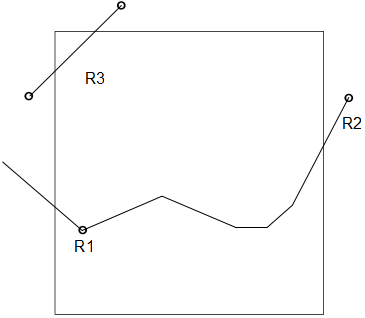
\includegraphics[width=120mm]{roadsRef.png}
\caption{Roads referenced by different points}
\label{fig:roads}
\end{figure}

 When searching in this range, all the roads should be returned. With roads referenced as a single point, R2 would not be returned, but R1 would. R3 would never be returned, even when referenced by two points. To solve this, an extra part of the map could be loaded, increasing the width and height of the rectangle by x, where x is the longest road in the map. Of course this would be inefficient if the roads' length is not systematically broken down, and this would require the data to be restructured. To be able to guarantee that all roads within an area are shown, we will need to take this approach for that particular solution.\\
The node has references to the roads that it is a part of. Storing nodes in the data structure has the same problem as storing roads referenced by two points. The difference is that nodes require more memory because an object is created for each one, but it makes the data structure contain less elements. As there are fewer nodes than road endpoints, it makes the kd-tree (discussed later in this chapter) more shallow, and therefore faster.\\
The most important requirement for our data structure is that it should be fast, while memory usage and start up time is less important. When looking at smaller parts of the map the improvement should be most significant. We chose the kd-tree because its binary structure and adaptive construction makes it efficient to access data, no matter how much it clumps(how numerically close the keys are to each other). While grid-file is potentially faster, the kd-tree is stable and does not depend on bucket size or other factors such as cluttering.  The Quad-tree data structure is also a viable choice to consider. The Quad-tree is potentially shallower, but it does get deeper when the data clutters. Empirical testing with both solutions reveals that a perfectly balanced kd-tree have a depth of 20, while the Quad-tree have a maximum depth of 52 on this data set. One of the kd-tree’s weaknesses is to return data from a rectangular query, which our aspect ratio does not allow, making it very suitable for our problem. We chose nodes as data objects because it is easier to implement, but to our best knowledge, roads referenced by one point should be the fastest and best solution.\\
\\
The algorithm used to search in the kd-tree should be as fast as the kd-tree allows it to. The data structure has an associated algorithm, which runs in logarithmic time making it very suitable for large data sets.\\
Construction of the kd-tree requires a median finding function, which is used for balancing the tree. The algorithm is not required to find the median, but it makes the tree shallower the closer it comes to the true median. The choice is either a median finding algorithm that runs in amortized linear time or an algorithm based on random picking elements to sort and find the median from. The first is much slower when constructing the tree, but makes the search faster. Empirical testing reveals that the difference in search time is very small when switching between the two ways of constructing the tree. Because the difference is small when searching and big when constructing the tree, we chose the random algorithm.\\

\paragraph{Searching for a route}
When we first started to discuss how we were to create an efficient way to find a route, we considered several ways how to approach this. One of our main concerns was to not let the user wait too long. To ensure this we figured the cost of this was to use some more memory instead. 

We considered several algorithms like DFS, BFS, Union-Find, but none of these were able to tell us the shortest path from A to B – only that there could be a path from A to B. The only two algorithms that actually would fulfil our needs was Bellman-Ford’s or Dijkstra’s algorithms. These two would be able to find the shortest path from any given point to another. 

Both of these uses a graph. As far as we were concerned there was two possible graphs we could use: An edge-weighted-graph or an edge-weighted-directed-graph. But since a one way road or a road were no driving are allowed could occur, we naturally chose the directed version, instead of adding a flag at the undirected graph to tell the driving prohibitions. Now we just had to decide whether to go with Dijkstra’s or Bellman-Ford’s algorithm.
The Bellman-Ford algorithm is able of using edges with a negative weight, but it performs slightly slower than the  Dijkstra algorithm, because it is forced to check for negative cycles. Because of our performance requirements, it was a problem that Dijkstra (as well as Bellman-Ford) would search the entire graph to find the distance from the starting point to every single node. Unless the user would search for the longest path possible every time, we had to be able to stop the algorithm when the destination had been reached. This would be quite easy to implement in Dijkstra’s – and considering the above, we decided to go with Dijkstra’s algorithm.

Another possibility was to let Dijkstra’s algorithm run from every node in the graph without stopping it. Then all these could be stored in an array, so we quickly could tell the user the fastest route. This would require an insanely amount of memory! Especially if the user had to choose between the fastest or shortest path.

Dijkstra's algorithm finds the shortest path, from one node to another, which does not solve the problem alone. To search from a arbitrary point on an edge, additional functionality has to be applied. We have thought of two solutions (see figure \ref{fig:routeFinding}). 

The first solution is as follows. When the user asks for a route between two addresses, the program finds the two edges which matches the addresses. Then the program selects the first node from the first edge and the first node from the second edge. The program then finds the route and if the route doesn't contain the edges that represents the addresses, the program then adds the edges to the route. After that the program calculates the right distance for the two edges that represents the two addresses.  This approach may show the wrong road because the first node to the the edge is always used in the route and there might be a shorter route that doesn't contain that node. 

The second solution is as follows. Instead of always selecting the first node for route finding the program should select the node that is closest to the given address. If the shortest route then contains the edge where the address is located the program should calculate the longest distance, otherwise it should add that road and calculate the short distance.

We decided to implement the first solution, but we found out later that it could show the wrong route. \\

\begin{figure}[H]
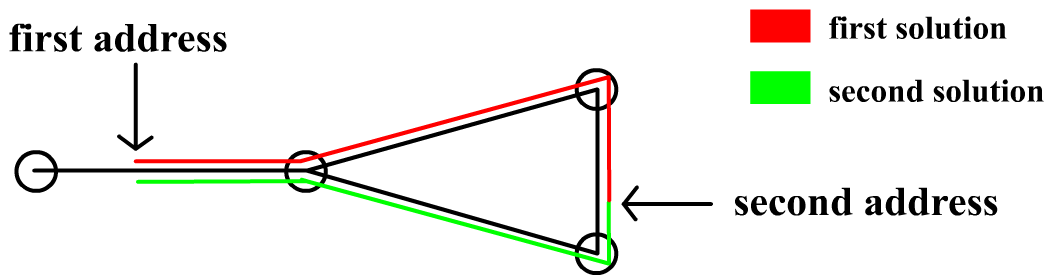
\includegraphics[width=120mm]{routeFinding.png}
\caption{Two different approaches to find the shortest path.}
\label{fig:routeFinding}
\end{figure}

			\subsubsection{User Interface}

				In this section we will discuss different ways that the user interface could be implemented. We will start off by discussing the overall decisions such as which technology we should use to show the data graphically. After that we will move towards a discussion of the features we will implement and how it should be done.  

The requirement for the user interface is formulated in the project description as follows: "Design a coherent user interface, which includes the map, but probably also other components". To fulfull this requirement we have to first of all select a technology to show graphical data for the user. In our case there are two obvious options. The first one is to use Swing and the other one is to make a browser based solution. In the following we will discuss both solutions.

\paragraph{Swing Solution}\mbox{}\

We will mention two advantages of using the Swing API. First advantage is that we will be able to use an advanced programming language. Using Java rather than Java Script will i.a. give us typesafty, a comprehensive standard library, chance for errorhandling and inheritance just to mention a few. The second advantage is that it will be easier to implement extra features because we already know the Java language and the Swing API. Using Swing also have som disadvantages and we will mention two. The first disadvantage is that the user will need a JVM to run the program. It is not difficult to download and install the JVM, but it is more convenient for the standard user to use a browser. The second disadvantage is that if the entire functionality is located in one program then the user will experience a long waitingtime every time the program starts up. Contrary there will be no startuptime for the user when using the browser solution. 

\paragraph{Browser solution}\mbox{}\

For the browser solution we will also mention two advantages. The first one is that long startup time and memory usage is acceptable for the server part because this part is running on a powerful computer and the user will not experiece this startuptime. That gives us the possibility to favor performance over memoryusage. The second advantage is that we will acquire knowledge about javascript, xml and svg, which are widespread technologies. We will also mention two disadvantages. The first one is that we have limited acces to the implementation. We don't know how the different browsers implements the different svg commands and therefore we have no possibility of improving performance in that part of the program. The other disadvantage is time consumption. Chosing a browser solution involves knowledge about a wide range of technologies such as HTMLl, CSS, Javascript, XPath, XML, SVG and HTTP. None of the group members had in depth knowledge about these technolgies beforehand.    

Based on the different advantages and disadvantages we have chosen the browser solution. The fact that we can focus on performance rather than memoryusage, that the browser solution is more userfriendly and that we get the chance to learn new technologies leads us to that descision.

\paragraph{Features}\mbox{}\

The second step in fulfilling the above mentioned requirement is to analyze how we, by using a browser, can make a coherent userinterface. Therefore we have to discuss which features should be implemented and how these features should be implemented, e.g. decide how much of the functionality should be located in the browser and how much should be located at the server. In the following we will discuss the different features.

\paragraph{Road displaying}\mbox{}\

To show the roads we have the option of using plain Java Sript or to use a combination of Java Script and svg. The advantage of using plain Java Script is that we would have the abillity to completely control the drawing of the roads and maybe optimize performance. The advantage of using SVG is that SVG supports a wide range of functionality and therefore we could save some time. Futhermore SVG seams to become a widely recognised technology, which means that more people might be able to understand and use our program in other contexts. Our choice fell on the combined solution with both Java Script and SVG. 
 
\paragraph{Scalable Map}\mbox{}\

The map needs to be scalable when the user drags the window of the browser. In our case that functionality comes for free when we use SVG. The only thing we need to consider is how SVG should show the map. Basically there are to ways (See figure \ref{fig:mapSliceMeet}). One way is to always let all of the viewport be visible no matter what aspect ratio the user will create when dragging the window (referred as "meet" in the SVG language). This will create a white border in the top and down or in the left and right. Another way is to cut of the map so that the map always takes up all the space (referred as "slice" in the SVG language). We chose the last solution because it makes use of all of the available space in the browser window and thereby utilise the users screen optimal. The only disadvantage is that when the user use the routeplanning, some of the route might be sliced off. This however could probably be fixed writing a SVG command that specifies the route's area and tells the browser not to cut off anything in that area.
\begin{figure}[H]
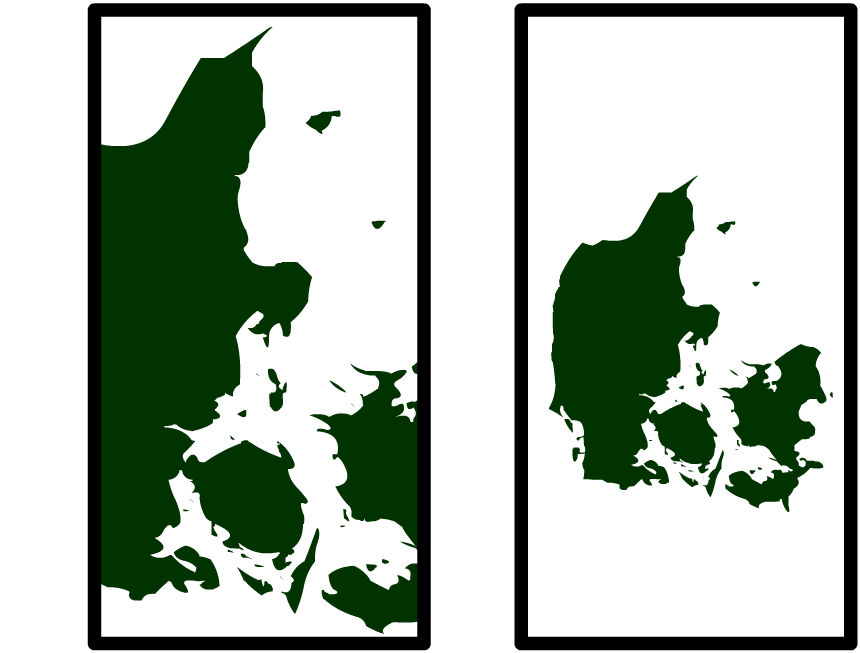
\includegraphics[width=100mm]{mapSliceMeet.png}
\caption{Illustration of the scale options. To the left a figure illustrating the "slice-option" which we chose and on the right a figure showing the "meet-option".}
\label{fig:mapSliceMeet}
\end{figure}


\paragraph{Zoom and Panning}\mbox{}\

When discussing zoom and panning there are two aspects. The first one is to consider how much extra data should be passed from the server to the browser. We have chosen to call that extra data for buffer data. When choosing the amount of buffer data there are two extremes. The first one is to let the browser request exactly that amount of data that the user is requesting. This way of doing it would make sure that it would be easy to develop a new view, e.g. a smartphone app, because most of the functionality is located at the server. On the other hand the user might experience the program as slow if the user has a slow internet connection. The other extreme is to let the browser request all data in one call and only show what the user is asking for. This would require a lot of functionality in the view, but it might result in a good experience for the user if the internet connection is slow. We have chosen a compromise where the browser request buffer data for panning and not for zooming.
The other aspect is to decide in what way the user should be able to zoom and pan. Since we know that it takes a long time to get the Java Script, HTML, SVG and XPath to work together we have chosen to settle for buttons in the browser as the only way for the user to navigate in the map. One could consider to make it possible for the user to use keyboard shortcuts and mouseevents for zooming and panning. 

\paragraph{Route Displaying}\mbox{}\

There are to different approaches of showing the route when the user zooms or pans after a routesearch. The first approach is to request the server for more map data and the same route. This approach is good because it keeps functionality at the server but it can be slow if for instance the user asks for a route from Copenhagen to Skagen, because the Dijkstra algorithm would run every time. The other approach is to save the route in the browser, which is relatively uncomplicated when using SVG. The last approach is the one we chose.	

				
				
		\subsection{Summary}
Through this analysis and these design choices, we have chosen a way to develop a program that meets the given requirements, and follow our own guidelines for what we want to focus on.\\
We have decided to utilize two different data structures. The Kd-tree will support the visualization of the map, and the graph-structure the route-finding. They will do this sufficienty fast, and as this is one of our main priorities, it outways the high memory usage of using two data structures. It will also allow for better optimization for both tasks, instead of forcing compromises. The vizulisation will be supported by the Kd-tree's range searches, and prioritizing of roads, while the Dijkstra's Shortest-Path-algorithm will utilize the directed edges of the graph.\\
Our choice of graphical-visualization will further support these tasks and requirements. The browser will be able to show all the roads with SVG, and use the build in viewbox to zoom and pan around the map. This also gives us a map that scales well with the window size. Through our method of sending data between the server and browser, we have tried to optimize for speed even further.\\
We will use a simple, user friendly UI with buttons to give the user control over these features, and input fields to choose addresses for route-finding. The buffer data will help smoothing out the load times, and again give the feel of a fast program.\\
With these design choices we have made a solution, that consistently focus to overcome the same major obstacles in each part - performance and simplicity of user interaction.
			
	\newpage		
	\section{Technical description}
		length : 0.5 - 1 side\\
		Her beskrives kort hvad der kommer til at være i det kommende afsnit..
		
		\subsection{Flow description}
		When the java-program is started, the Loader class begins loading the text files, which contains the necessary information about Denmark’s infrastructure. The Loader holds the information in suitable collections until other parts of the program is called from the controller. The kd-tree builds the tree structure from nodes and the graph is built from the directed roads. From there on, the program listens for browser requests, returning xml files containing roads from a region of the map and possibly a route.\\
When a user of the application wants to see a part of the map, a request is send to the java server, which is first caught by the JSConnector class.  The connector component gets the information for the client from the Controller, which gets information to complete the request from different components of the program. The KDTree and RoadSelector classes retrieves the relevant road objects, while the Routing component finds the route if it is requested. When the region and route information has been generated it is send as an xml in String form to the client. 

		\subsection{UML Diagram}
		The following UML diagram is a selection of the most important classes, for instance most of the exception classes have been left out for better readability. Also, for clarity, not all of the relationships (symbolized by arrows) between classes have been drawn because some of the classes are used primarily for storing data and are therefore used in many classes. 
		\begin{figure}[H]
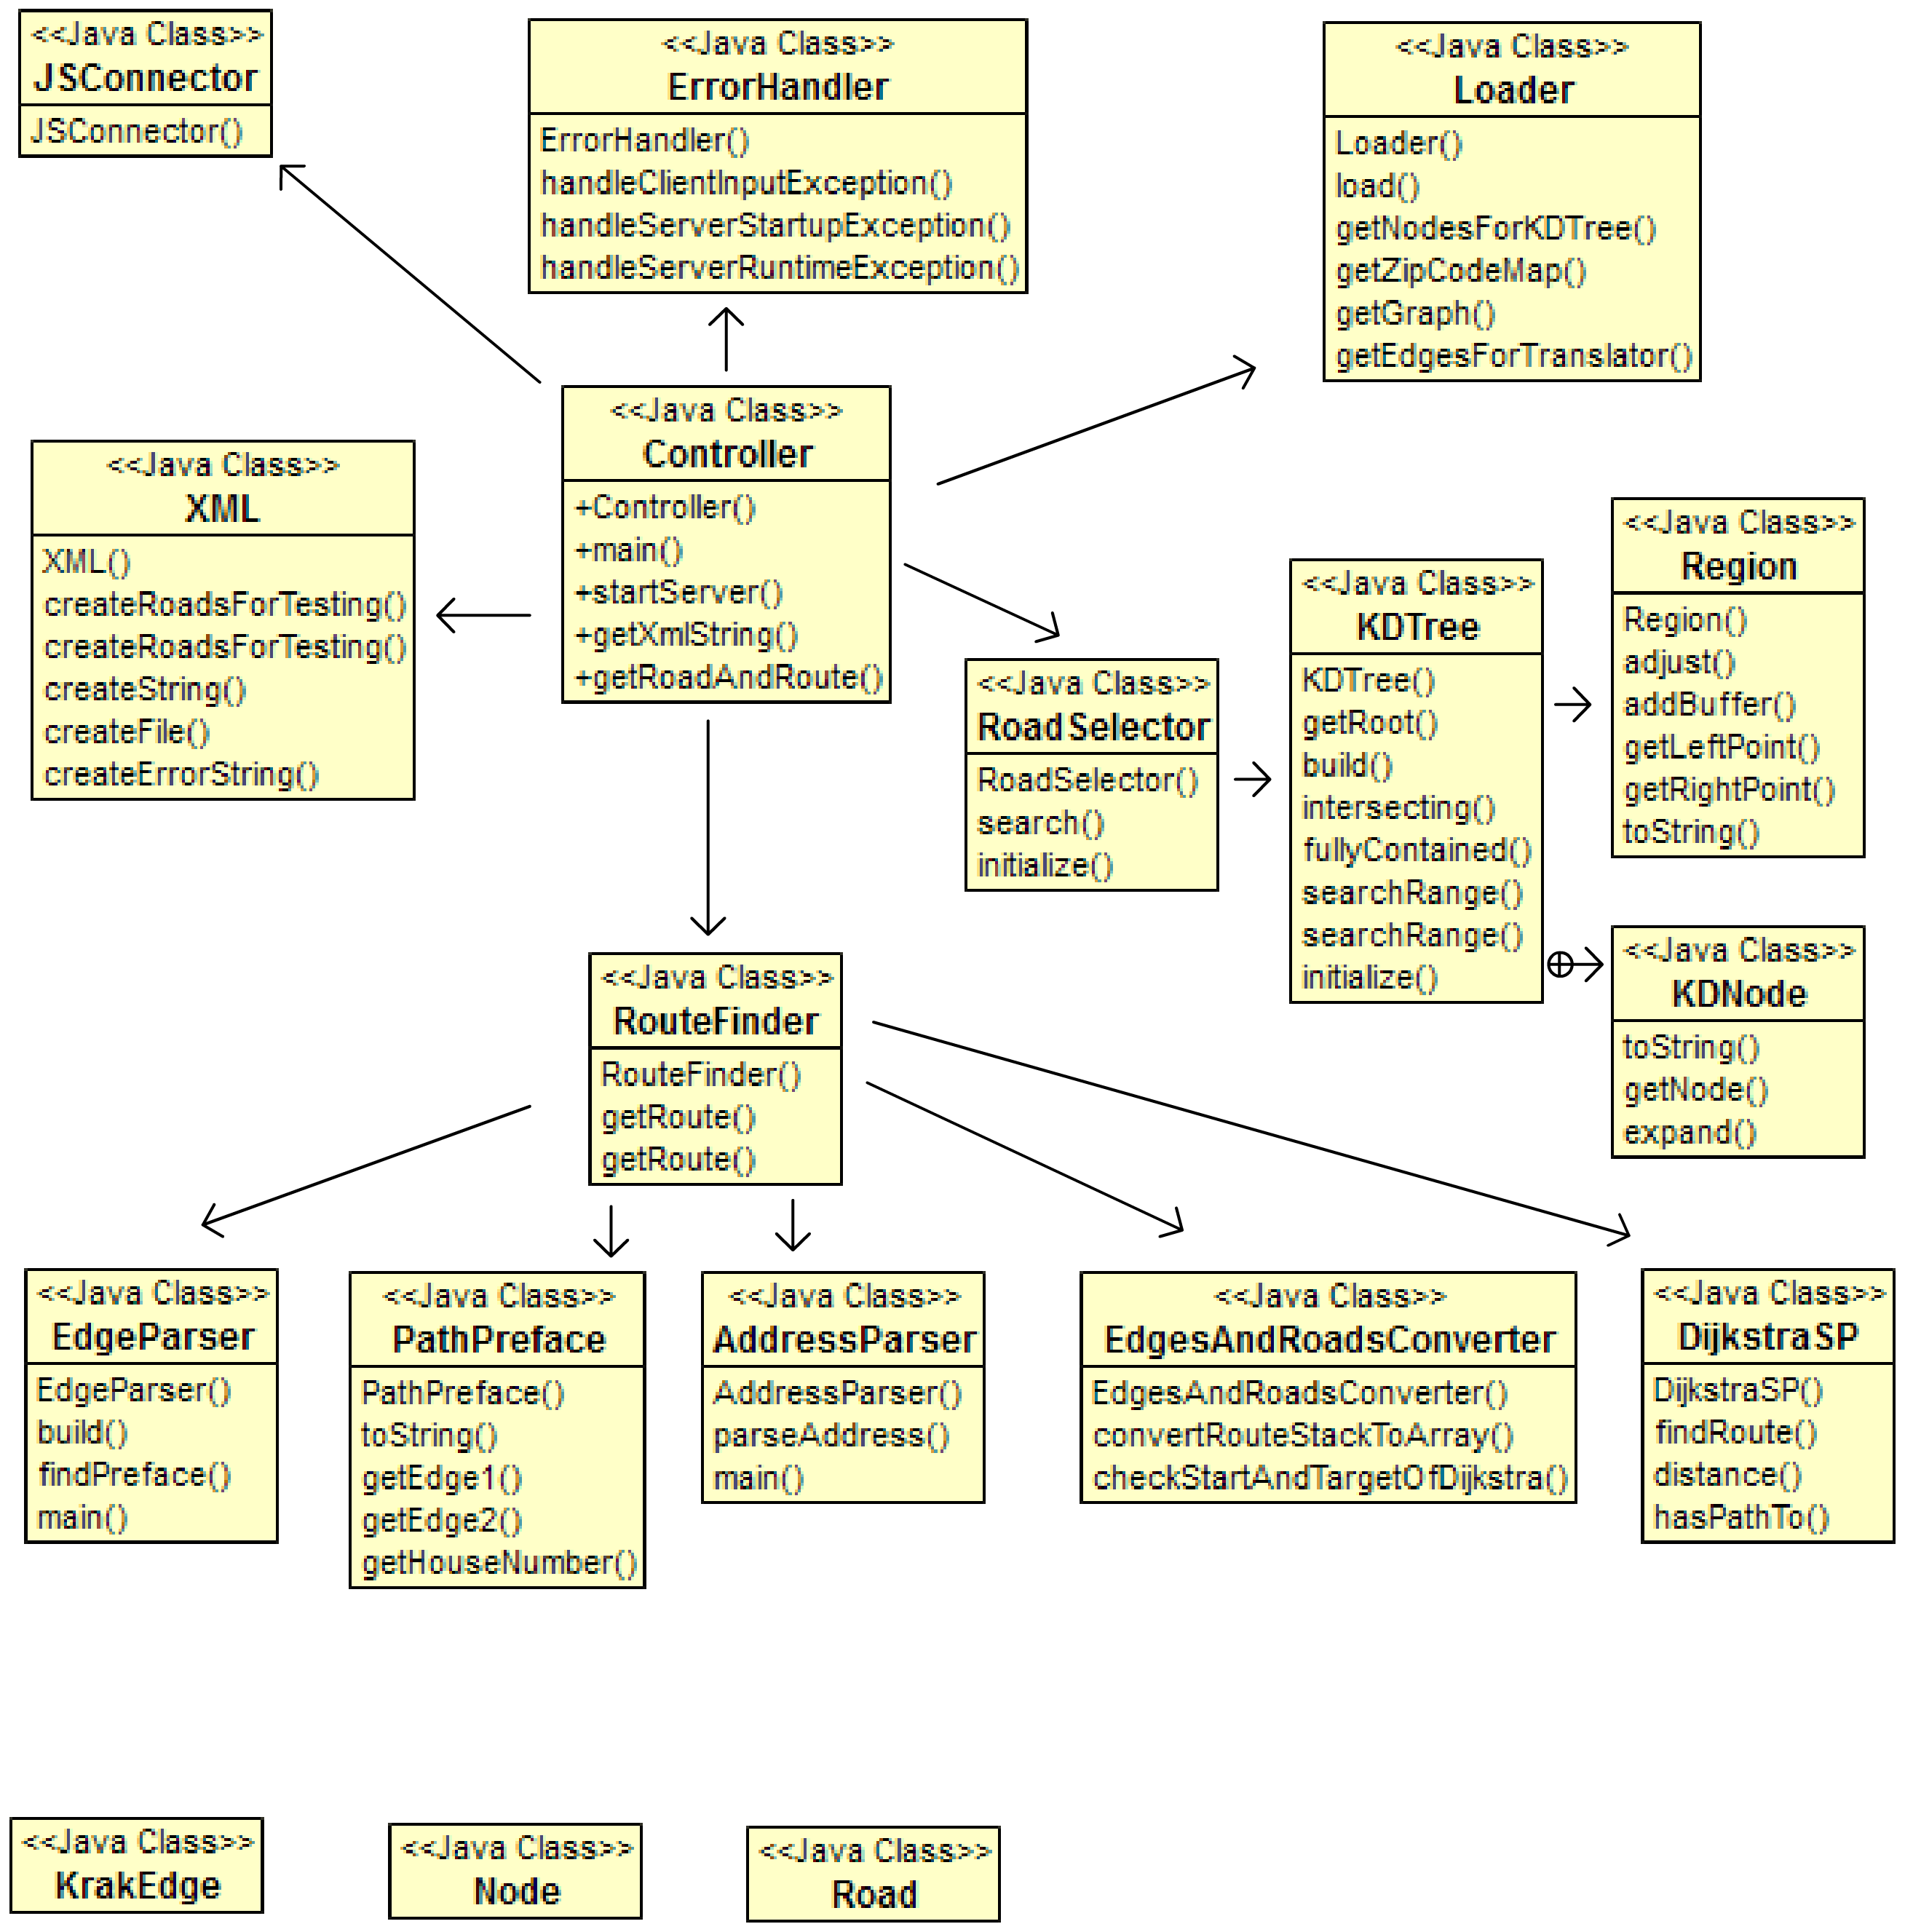
\includegraphics[width=120mm]{umlArrows.png}
\caption{UML diagram showing the most relevant classes.}
\label{fig:uml}
\end{figure}
		
		\newpage
		\subsection{Classes and responsibility}
			length : 0.5 - 1 side\\
			Kort beskrivelse af hver klasse plus deres ansvar\\
			
			\subsubsection{Controllers}
			
				\paragraph{Controller}\mbox{}\
				
The Controller class is the main unit and the one to connect all the classes to a functioning program. It will never compute any data, but simple send the requests/data back and forth.  This is also the reason why all methods and fields are static.\\
Since the program, at this point, is rather simple it only contains a few methods. All it needs to take care of is the starting of the server, getting a part of the map or getting both a part of the map and a route. When the class starts up the server, it specifies what files to be loaded into the Loader, and after this is done, the rest of the classes which also at some point need to be initialized is done. Hereafter the RoadSelector and the EdgeParser are initialized.\\
If the Controller is asked for a XML request containing a route, it will use the RouteFinder to return an array of Roads that represents the route. After this, the region to be shown on the map is chosen by a getter in the Road class that tells in what region the route is in. This will be used to select the appropriate region of roads by the RoadSelector.\\
Now the Controller sents all these informations to the XML class and forward the returned String to the JSConnector.\\


					
			\subsubsection{Error handling}
				
				\paragraph{ErrorHandler}\mbox{}\

This is the main class of the system responsible for errorhandling. When the Controller gets a propagated Exception, it calls one of the three main methods in this class; handleServerRuntimeException, handleServerStartupException or handleClientInputException. The first two methods will print out the StatusCode relating to the current Exception, by calling getDescription from the getStatusCode method in the exception. Furthermore the handleServerStartupException will try to make sure that the Java virtuelmachine is terminated properbly.\\
The handleClientInputException will not make a print out of the description of the StatusCode, but return it to the Controller, for sending information to the client.

				\paragraph{StatusCode}\mbox{}\

An Enum-class. Responsible for converting a Enum of a given Exception into a StatusCode-number, and a description of what error this number relates to.
				
				\paragraph{ServerRuntimeException}\mbox{}\

An abstract class that extends Exception, to act as superclass for any ServerRuntimeException. Has methods for storing and returning the old, original Exception thrown by a class in the Java-libraries, and an abstract method for getting the StatusCode of the new Exception.
				
				\paragraph{ServerStartupException}\mbox{}\

An abstract class that extends Exception, to act as superclass for any ServerStartupException. Has methods for storing and returning the old, original Exception thrown by a class in the Java-libraries, and an abstract method for getting the StatusCode of the new Exception.

				\paragraph{ClientInputException}\mbox{}\

An abstract class that extends Exception, to act as superclass for any ClientInputException. Has an abstract method for getting the StatusCode of the new Exception.

				\paragraph{LoaderFileNotFoundException}\mbox{}\

A class extending ServerStartupException responsible for wrapping Java's FileNotFoundException in the Loader. Thrown if the files with the dataset could not be found.

				\paragraph{XMLTransformertException}\mbox{}\

A class extending ServerRuntimeException responsible for wrapping Java's TransformerException in the XML class. Thrown when the Document could not be properbly transformed to either an XML-string or to a file.

				\paragraph{XMLDocumentException}\mbox{}\

A class extending ServerRuntimeException responsible for wrapping Java's ParserConfigurationrException in the XML class. Thrown when the Document could not be properbly build.
				
				\paragraph{AddressInputFormatException}\mbox{}\

A class extending ClientInputException. Thrown when the input format of an address, does not match an regular expression.

				\paragraph{NoSuchRoadnametException}\mbox{}\

A class extending ClientInputException. Thrown when the input roadname could not be found in the database.
				
			\subsubsection{Models}
			
				\paragraph{KDTree}\mbox{}\
				The KDTree class is responsible for creating the data structure and implementing the search algorithm for range searches. The KDTree contains nodes, which are the input and output type. The KDTree gets its input nodes from the Loader class. The output from the search function is used by the RoadSelector class.\\
Creation of the data structure is done by calling the expand method on a KDNode object, which will construct the tree recursively. The KDNode is a nested class, which serves as a container for the real node object. Each KDNode has references to its child nodes, the left is smaller than the nodes relevant coordinate and the right one is greater or equal to. The expand method finds the median node from the input collection and returns that node as the child node. It calls the same method twice, each with approximately half of the collection it was given, divided by the median node. By changing the axis, which the median is calculated from, a two dimensional tree is constructed.\\
Searching in the tree is done from a region input. When visiting a node, a region is defined from the axis, which the node was chosen as median from. For instance the first node (root node) defines two regions that ranges from the largest to the smallest y-coordinate. The left region for this node ranges from the smallest x-coordinate to the nodes x-coordinate and the right ranges from the biggest x-coordinate to the nodes x-coordinate. For both regions the geometrical functions fullyContained and intersecting investigates how they relate to the input region. If the region is fully contained in the input region it returns all child nodes. If it is intersecting, this function is called recursively. This logic makes the function investigate regions that are intersecting the input region, exclude regions that are not, and fully include regions that are a part of the input.

				
				\paragraph{Loader}\mbox{}\
The overall purpose of the Loader class is to load the Krak data from three textfiles and on the basis of the textfile it creates four data structures: a list of nodes used to build the KDTree data structure, a graph to be used by the DijkstraSP class to find the shortest route, a list of edges to be used by the EdgeParser class to translate a user-typed address to an Edges object and the last data structure it creates is a map of zip codes which is also used by the EdgeParser class.\\
In addition to loading the textfiles and making data structures the Loader class is also responsible of repositioning the nodes' coordinates so that the upper left corner of the map is located in 0,0.

In the following we will describe the class in details. The first text file to be read is the node file. Each line is read one at a time and for every line a node is stored in a collection. The class iterates through the collection and finds minimum and maximum for x and y values. After that the class iterates one more time through the collection and calculates a new x and y value.  

When the node file have been read the class continues and reads the edge file. This file is also read one line at a time and for each line a KrakEdge and a Road object is created. The KrakEdge gets all the properties from the file and it gets a x and y value from the matching nodes. The Road object is being referenced to the matching nodes so that the KDTree class later on will be able to return the appropriate map section. The last thing that happens in the Loader class is that the KrakEdgeWeightedDigraph class is being instantiated and all the edges read from the text file are being added to that object. 

				\paragraph{Node}\mbox{}\
				
				This data class is an representation of geographical points which are connected to each other with road segments. These Node objects are constructed in the Loader using the data in the supplied Krak data files. 
				
				\paragraph{NodeComparator}\mbox{}\
				
This Comparator is used when building the KD-tree. It compares a specific coordinate of two nodes to decide which one is higher and lower(Hvorfor er det interessant?). The coordinate can be chosen at the time the object is constructed(Hvad mener du med det?).

				\paragraph{PathPreface}\mbox{}\
				
The class represents a system specific line of an real address. Since the graph that we have implemented is a directed graph, there can potentially be two edges for each road segment, one going each way. This object consists of up to two KradEdges, and a house number specifying which road segment the PathPreface object is representing.

				\paragraph{Region}\mbox{}\
				
This data class is a representation of a square region, defined by 2 two-dimensional points. These two points are the coordinates of the opposite corners of a square.
				
				\paragraph{Road}\mbox{}\
				
The Road class is a data object to represent a straight piece of a road. It will contain information of the roads type, name, starting point, ending point, hashcode and priority. Beside these values, there are stored 2 static HashMaps, to set what color and width a road object shall have depending on the value of its type. \\
The top and origo for the current selection of roads are also stored in here as static fields. These are set when a route is found, so that the Controller knows which region to use when asking for a section of the map
If the server was to take care of concurrency, this would be one of things there had to be changed, because it would be able to set an unfitting viewport to a client.\\
Last but not least, the type to define a road as a part of a route is set in here. In that way all the relevant information about what color and width a certain road should have is stored at one single place.\\
A final thing to notice about the Road class is that it stores only some of the information of the actual road compared to a KrakEdge. This is to spare some memory use and hopefully make the program a bit more smooth.\\

				
				\paragraph{RoadSelector}\mbox{}\
				
This class is a result of keeping the KD-Tree as a purely data structure class. It adds additional functionality when it comes to determining what Road objects to show to the user, based on a given Region. It offers additional filtering based on prioritising different Road types.\\
The RoadSelector class gets a collection of nodes as output from the KDTree. To get a collection of roads, it iterates trough every node object and collects the roads, which the node has references to. With this technique, a lot of duplicate road objects exist. To solve this, we collect the roads in a HashSet, which only allows one instance of every object. As the HashSet handles up to a half million roads, it has been subject to optimization. Different load factors (The percentage amount of the collect that is filled, before it is resized and rehashed) and initial capacities have been empirically tested.\\
The hashCode function of the Road class has been automatically generated by eclipse, and are calculated when the road is made. This is to save operations when the road is filtered by a HashSet and it is correct because the Road objects never are changed after they are made.
				
				\paragraph{RouteFinder}\mbox{}\
				
The RouteFinder class is used only to get a better and more organized design: It keeps track of all the classes used to find a route, all the way from the input of two address Strings, or two PathPrefaces, to the output of an array of roads, which contains all the Road objects representing the route. During the computing of the route, the RouteFinder will first find the corresponding PathPrefaces to the addresses. Then it instantiate DijkstraSP with our directed graph, which is weighted by edges, and uses Dijkstra’s searching algorithm to find the shortest path from a random end of the start edge to a random end of the ending edge in the route. This will later be checked to see that the correct starting and ending edge is found.\\
After this the first and last edge will be replaced by a new edge, that will be shortened to start or stop by, where the house number probably will be. This is determined by the amount of house numbers at the edge and what house number the search provides.\\
RouteFinder is the only class that uses the following classes: AddressParser,  EdgeParser, DijkstraSP and EdgesAndRoadsConverter.\\


				
				\paragraph{XML}\mbox{}\
				
The purpose of this class is to create a XML file, which can be converted to a String and returned to the client. The class contains code which creates XML elements, as for instance roads, route, viewport or statusCode, and will put these into the correct place of the XML structure. It will fill the groups with data taken as parameters from the method signature. \\
One thing to make sure when creating a new Element is to use the same document for which it will be appended to later. Because of this a Document is created in each start of the method and send as parameter to the private methods, which is made to avoid duplicating code.\\
The method createErrorString is used if something go wrong during the creation of the XML. In this way the server will still be able to send some kind of notification to the client and improve usability.\\
The last method called createFile is made for debugging, to see what actually is sent to the client.\\


				
			\subsubsection{Routing}\
			
				\paragraph{AddressParser}\mbox{}\
				
This class is responsible for interpreting a String and sorting it into a array of Strings. It uses regular expressions to identify the road name, road number and associated letter, postal code and city name.
				
				\paragraph{DijkstraSP \cite{sedgewickAndWayneDijkstraSP}}\mbox{}\
				

This class has been copied from Sedgewick and Wayne and modified to fit our program. \\
DijkstraSP responsibility is to find the shortest path from one node to another. When the class is instantiated it takes a KrakEdgeWeightedDigraph object as a parameter, which is statically stored in Loader. When the method findRoute is called, Dijkstra’s algorithm is performed on all nodes until it reaches the destination node. We have chosen to stop the algorithm here to get a better performance and the rest of the computing will never be used unless a new search is called – and it will start all over again, since the start node is most likely to be changed and therefore the previous data can’t be reused.\\
When the route has been computed and should be returned, it will follow the computed route backwards to add it all up in a Stack to make the returned route come in the right order.\\
Since the graph is made from a real set of roads, there can be no negative roads. This is also one of the reasons why we choose Dijkstra: It’s faster but cannot be used for negative edges.\\
DijkstraSP will use some specific versions of Bag\cite{sedgewickAndWayneBag}, In\cite{sedgewickAndWayneIn}, IndexMinPQ\cite{sedgewickAndWayneIndexMinPQ} and Stack\cite{sedgewickAndWayneStack} (not the one from java.util.) to be functioning. These classes have also been taken from Sedgewick and Wayne and will not be mentioned elsewhere.\\
 
				
				\paragraph{EdgeParser}\mbox{}\
				
This class associates road names, numbers, postal codes, and city names with the correct directed edges in the graph. This is used to find a specific object based on the user search input.
				
				\paragraph{EdgesAndRoadsConverter}\mbox{}\
				
This class is used as a part of our route searching system. It only has two purposes: The first is simply to transform a Stack of KrakEdges into an array of KrakEdges and the second is to make sure the correct start and target KrakEdge is used.\\
To make sure that the correct start and target is used in the route the class is taking care of adding the correct KrakEdge if it is needed. This is done by comparing the first and last edge to the KrakEdge it is supposed to be – if they are equal nothing will be done else the supposed edge will be added.\\
Then the length of the first and last edge will be computed to a length that approximately correspond to where the houses are located. This is calculated on the basis of the house number the user is searching for compared to the amount of house numbers on the edge.\\
Another important thing this class takes care off is to determine what view that will be showed to the client. When the route is found and corrected, it will be transformed to a Road[] and at the same time the class will find the minimum and maximum values for the routes coordinates. After that it will be set to the static field in Road, to be used when finding the other roads to be displayed and set in the XML sent to the client.\\


				
				\paragraph{KrakEdge \cite{sedgewickAndWayneDirectedEdge}}\mbox{}\
				

This class has been copied from Sedgewick and Wayne and modified to fit our program. The KrakEdge is a data object, representing a straight piece of road and used when searching for a route. It carries a lot more information than a Road object, like information of the house numbers or postal codes. One thing to notice is the static field isLenghtWeighted; which is used for knowing whether the weight of the route should be weighted by the length or travel time. The only method that can set anything is also just for this single field. For the rest of the class it consists of purely getters, since we take it that a road only can be changed if the server is restarted.\\


				
				\paragraph{KrakEdgeWeightedDigraph \cite{sedgewickAndWayneEdgeWeightedDigraph}}\mbox{}\
				

This class has been copied from Sedgewick and Wayne and modified to fit our program. The KrakEdgeWeightedDigraph contains one of our data structures, which is used when searching for a route. It is a directed graph that contains information of how many nodes there are and how many edges there are leaving from each node. This is the reason why it for instance can distinguish a one way road from a road with no limitations. Furthermore the nodes are bases on numerical id’s which fits our program perfectly since the edges from the data files also are based on numerical id’s. \\

				
			\subsubsection{View}
			
				\paragraph{JSConnector}\mbox{}\
				
				This class is responsible of listening for requests from the browser. When the class receives a request it parses the url string. Based on the parameters it either calls a method for receiving map data only or it calls a method for receiving both map data and route. The class then returns the resulting xml string to the browser. 
						
				\paragraph{index.html}\mbox{}\
				
				The index.html file contains both HTML and Java Script. The HTML part is responsible of positioning the map element, the buttons and the text fields. The Java Script part takes care of connecting to the server, adding the received SVG element to the HTML DOM, maintaining the viewport when the user zooms or pans and it takes care of receiving errors and displaying the right errors to the user. 
		\newpage	
		\subsection{Errorhandling}
			A good idea to handle exceptional conditions and errors in a program is to form somekind of strategy or policy. This helps to a more streamlined error handling
			when the program is written, but also if the program is to be expanded at some point. A very simple policy that one could decide, is to
			simply handle the exception exactly where it's created. This would be easy to implement and since this is the most standard way of dealing with
			exceptions, most programmers would know this policy and therefore wouldn't have any objections towards it. On the other hand, it is hard to see, from
			the outside, where and how an exception is handled and therefore also very hard to make a real policy for, specially when it comes to expansion.\
			When starting to form such a policy, one very central thing, is the ability to predict which kind of errors and exceptions that can and will 
			occur in the program. We have divided our errors and exceptions into tree areas. There is always a potential of startup-files missing, a loss of internet and many others like these two, that can cause a server to being unable to start. All this is put into the area of 'startup'-errors. The next area are errors that can happend any other time after the point of startup. These a called 'server-runtime' errors. This could be a case, where the program usage of ram exceeds the allowed maximum. The last is called 'client'-exceptions. These types of exceptions can only be caused by the client. This could for example be bad input or missing input.  Because of the different times that errors and exceptions can occur and the level of criticalness, it's clear that they each require different handling. \
			To overcome this we will make a hierachy of exceptions classes, each for one of the tree types of errors. The idea with our own exceptions classes is that we will 'wrap' the actual exception and pass one of the above mentioned exception to a central errrorhandling class, which will hold the responsibility of dealing which all exceptions. This will remove errorhandling responsibility from both the actual class, where the exception is thrown and from the controller class, which only passes the exceptions to the errorhandling class.\
			In the errorhandling class will be tree types of methods and a reference to an enum class called 'StatusCode'. Since we need to handle the tree types of errors different, we decided to do so, by having tree different methods. For example no matter what kind of server-runtime exception the errorhandler class receives, it will always deal with it the same way, since it always will be the method for server-runtime exceptions that are called. The same goes for the two other exceptions classes.\
			The advantages of doing it this way, is the overview that it gives and the /* OMFORMULERING easy way of expanding the system*/. All exceptions will be located in the StatusCode enum and inside the errorhandler class it's possible to see how each type of exception is handled. Futhermore since every exception has to be wrapped inside our own exceptions classes, a programmer i forced to decide how a possible error or exception should be handled and then use either 'server-runtime'-, 'serverstartup'- or 'client'-exceptions. Then he will make a new statuscode for this new error and then the controller and errorhandler class take care of the rest.\\
		There are though some disadvantages. This system will only scale so far. At some point, even with the gathering of exceptions in a hierarchy, the system will clutter with to many new exceptions. But for a system such as ours, it is quite fitting, and a solution to the problem could be, to make additional error handling classes for each part of the system, to split some of the work out.\\
	\newpage
	\section{User Manual}
		\paragraph{Starting the Program}\mbox{}\
		The program is divided into two parts - a server and a client. To start the server you need to have the Java Virtual Machine installed on your computer. If the JVM is installed you can either click on the kf04.jar file or you can run the file using the command line by typing java -jar kf04.jar. If you click on the file you have to wait for about 15 seconds and if you run it from the command line the program will tell you when it is ready. When the server is ready you can open the index.html file in the Chrome browser. It is important to notice that the program is only optimized for Chrome and may not work on other browsers. If you try to start running the server when the server is already running you might get an error because because the port already is being used. The only way to handle that problem is to close the JVM and run the program again.  
		\paragraph{Using the Program}\mbox{}\
		
		To zoom in or out on the map you can use the button with the - or + sign and if you want to navigate around on the same zoom level you can use the up, down, left or right button. Do you want to find a route from one address to another you can type the first address in the first text field and the second address in the second text field and press the find route button. If you want to clear the route you press the clear button.

		 \mbox{}\\
		
		\begin{figure}[H]
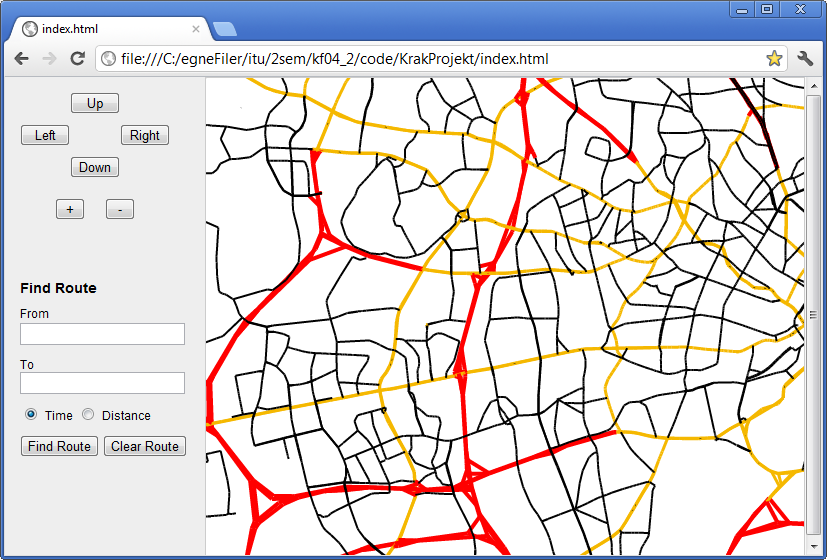
\includegraphics[width=110mm]{screendump.png}
\caption{Screendump of the browserwindow.}
\label{fig:screendump}
\end{figure}
		
		
	\newpage
	\section{Testing}
	When building our program we have to ensure that the code we have written actually works as intended. When the program compiles without errors, that is unfortunatly not a guarantee of the program working correctly. To ensure that it is functional in the way we have intended, we need to test it in several ways to see our code in action. Ideally we would have to check every component of our program in several ways, but this can be a very time consuming process. We have chosen to focus our testing on the parts that we felt are the most critical to the entire program.

Since our program is split up into different independant modules, getting to test different parts is a stright forward process. Most of these classes are tested after a philosophy much like a "BlackBox"-test. We test what the publicly accesible methods of the class return when given some example input. If the return values are what we expect them to be, we can somewhat assume that it is working as we expect it to. The example input can and should be all kinds of valid (and invalid) input. We do not only test situation in which we expect the class to function properly, but also situations in which we expect it to fail, so we can see how it reacts as well.

Few sections of the program have undergone a more thorough test, in which we comb every corner of the code to see if every line of the code is acting as we want it to, if conditional statements are checking the correct things, and wether branching is done correctly, among other things. We have restricted ourselves to only "WhiteBox"-test a certain few classes that are crucial, because it really takes up a lot of time. At this point in development we would have been better of using on other parts of the project.

If we had continued developing on this program, or if we extended the contents of our program substantially, we would have used more time on testing, and as a result, our testing methodology would be different. We could have made better use of JUnit to write and perform proper unit tests on our classes, and we would be more thorough with getting around and testing everything. It is generally recomended that you "test early, test often", and although we did test early in development, we have not been expanding the functionality of our program enough to justify testing more often. 

We have not choosen to include usability test in our testing, because the client interface is very simple, and we are aware of simple obvious improvements such as dragging, keyboard controls and map information.

	
		
		\subsection{Whitebox}
			length : 0.5 - 1 side\\
			
			Vi laver kun det her paa en del af programmet - hvorfor har vi valgt lige netop denne del?\\
			
			In this part there will be a description of how our whitebox test of the program has been conducted and what results we got from the test. \\
Before writing the actual test, there a several things to take into considoration. Is it necessary to test every line of code in the whole program and at what level do we want to do the whitebox test bit. The right thing to do, would be to test the whole program and make sure that there a no lines or statements that is not executed at least one time doing runtime. Since this would be very time consuming and because it's stated in the project description that it's not necessary to perform whitebox testing of the whole program, we have choosen to limit this to one single class.  \\
We have choosen our AddressParser class to be the target of our test. We have picked this class because of the many different scenarios that can happend when a user types an address and therefore is interessting to test and important, because of the criticalness of the address being parsed correct. One could argue for that other places in the program is equally important to test, but again, because of the limited time we have choosen only this place. \\
When doing a whitebox test there a several different levels and thouroughness of which the test can be performed. The least thourough way is to look at only the methods in the class. Are all methods executed at least one time? This would leave a lot of possibilities of statements and branches inside of some method, that wouldn't be executed. Therefore its also an option to look at every line of code, to see if all lines a executed at least ones. This would require a lot more time and work, but this way is more thourough. We have chosen a level, where we will test if all if-statements in the AddressParser in executed. \\

We started out by looking at all the methods and if-statements in the AddressParser and on the basis of that, we created some scenarios. These would make sure that we at all if-statements both had a scenario that would that turn the statement true and one turning it false. We chose input, and for these scenarios, and set them up in this expectancy table, categorized according to which private sub-method they belong to:

\begin{table}
\caption{table}
\centering
\begin{tabular}{c c c c c}
Method & Scenario & Input data & Expected output & Assertion result \\ [0.5ex] 
\hline
findRoadName & No valid road name & "123, 123" & "" & Success\\
findRoadName & Valid road name & "Langvej 5a, 5. sal, 2300 Kbh S" & "Langvej" & Success \\
findCityname & No valid city name & "123, 123" & "" & Success \\
findCityName & City name too short & "Langvej 5a, 5. sal, 2300 S" & "" & Succes\\
findCityName & 1 letter infront of cityname & "Langvej 5a, 5. sal, 2300 i Kbh S" & "Kbh S" & Success \\
findCityName & Valid city name & "Langvej 5a, 5. sal, 2300 Kbh S" & "Kbh S" & Success \\
findZipCode & No valid zipcode & "Langvej 5a, 5. sal, 123 Kbh S" & "" & Success \\
findZipCode & Valid zipcode & "Langvej 5a, 5. sal, 2300 Kbh S" & "" & Success \\
findHouseNumber & No valid housenumber & "Langvej" & "" & Success \\
findHouseNumber &  Housenumber with letter & "Langvej 5a, 4. sal, 2300 Kbh S" & "5" & Success \\
findHouseNumber & Valid housenumber & "Langvej 5 4.sal, 2300 Kbh S" & "5" & Success \\
findHouseNumber & Housenumber too long & "Langvej 2300 Kbh S" & "" & Success \\
findHouseLetter & Houseletter already found & "" & "a" & Success \\
findHouseLetter & No valid houseletter & "Langvej 5, 5. sal, 2300 Kbh" & "" & Success \\
findHouseLetter & Valid houseletter, no city name already found & "Langvej 5 a, 5. sal, 2300 Kbh" & "a" & Success \\
findHouseLetter & Valid houseletter, different from city name letter & "Langvej 5 a, 5. sal, 2300" & "a" & Success \\
findHouseLetter & Houseletter found, matching city name letter & "Langvej 5, 5. sal, 2300 Kbh S" & "" & Success


\end{tabular}
\end{table}

Then we used the JUnit test tool, to write tests to see if all our if-statements were executed and did match the expected results from our table. The expected results match in all cases. This assures us, that all branches of the methods have been reached properly, and acts according to our intentions, as the result output would not have come out as it did, if the call had not turned the if-statements the right way to true or false.


		\subsection{Blackbox}
		We have chosen to black-box test the kd-tree because its output is very important for the program to function. There are relatively few if-statements and “branches”, which makes white-box testing less relevant.
To test the output JUnit are used because it is an easy way to construct and run automated tests. As the kd-tree is one of the few places that has been subject to a lot of development, automated test have been beneficial. The expected output of the kd-tree is nodes, which lies in the input region. The linearSizeRequest function runs through all nodes and picks the ones inside the input region, which it counts. It is used to compare against, and is viable because it is very simple and therefore is less likely to contain errors.\\
As the input from the kd-tree is a region, there is an infinite amount of combinations possible. It is important to represent all kinds of inputs when testing, therefore the regions made to test the kd tree, represents both small and large regions, as well as regions that are in the north, south, west and east. The testing should reach all possible branches, which is done by both making regions that intersect and are fully contained in different levels of recursion.\\
The support functions, intersecting and fullyContained are also tested on borderline cases, even though we haven’t spent as much time thinking for this part of the testing, because a failure in the part most likely would lead to failure in the kd-tree output.\\

			
		\subsection{Errors, bugs and list of needs}
When requesting a large area of the map, the HashSet function sometimes uses approximately 8 times the normal time to filter the roads. As the error occurs differently on different computers, include classes implemented by java and is very hard to recreate, we have not been able to find the root of it.
\\
We do not take turn restrictions into consideration when finding the shortest path. This is a result of prioritizing other parts of the program.
\\
When finding the shortest path with a house number, the path-finding algorithm splits the edge which contains the house numbers to make it possible to navigate from the middle of an edge. However there is no guarantee for the correctness of this split, as the data set does not contain the necessary data for this operation.
\\
When searching for an address, the city name to zip code translator may make the request fail because one city district (København K for instance) can contain roads registered under different postal codes. The translator (EdgeParser) will translate the district to only one postal code.
\\
If a road is included in a region, but both of its reference points are outside the region, it is not shown. This is a result of choosing the data structure which is easier to implement.
\\
The region shown when showing shortest path does not include the entire route. This is a result of the way that the client adjust the viewport to match the aspect ratio, which the server does not know about.
\\
When panning the map 8 times in one direction, a white border may appear. This disappears when navigating the 9th time. We suspect that the root of the problem is a difference in the way the server and the client calculates the buffer.
\\
It is not possible for the user to navigate with the keyboard. This is a result of prioritizing other program functions, but if we had more time, we would make that work.
\\
The server is not able to handle rapid zoom requests in a satisfying manner. This could be handled by making a time delay after the user requests the zoom, where the client waits for another request to overwrite the first with. This would result in the server only answering once, and the user waiting less. If we had more time we would implement this feature.
\\

			
			
		\subsection{Results}
		Initially testing did not play a critical role in this project, because we did only find few errors in the classes we systematically tested. However testing made sure that these classes worked early in the development, which saved us a lot of time. When encountering a program error, finding the root of it is easier when certain parts of the program can be excluded from the error search. We had a lot of errors with the visualization of the roads, with could root in a lot of different classes. Having JUnit tests for the KDTree insured that it worked, which helped trace the bug.\\
		Because of the advantage testing gives, even without finding any bugs, we would have been better off testing more classes. Automated and manual tests would speed up the development of new features and would therefore be an essential fundament for expanding the program. 

			
	\newpage
	\section{Product conclusion}
	To review how the product meets both the project and specific requirements, it is assessed and compared from different perspectives. The product is able to navigate around the map and draw the roads in the viewport and filter them depended on cluttering and priority. It can find the shortest path from one address to another, but it does not guarantee that the path reflects a legally drivable route. The user interface is fairly simple, intuitive and easy to use. Whether the user interface is responsive, is very depended on witch part of the map the user is looking at. As the client is another thread than the server, the user interface itself is responsive. The program is not responsive when exploring regions that are greater than half of the map, but when zoomed in it runs with sufficient speed. It can take a second for the server to complete a request for the entire map. Requests for small parts of the map are completed almost instant(less than one hundredth of a second). There are many factors which contribute to this variation in performance, the primary being the data structure solution that involves a HashSet. Drawing roads with SVG has also shown to be much slower that other solutions such as Java Swing, making the browser another limitation in performance.\\
The specific requirements for the project, discussed in the problem analysis, have partially been reached. One of the requirements was making the basic functions work well and fast, which has been done, apart from navigating big parts of the map. The shortest path algorithm runs with sufficient speed, and by making the client save the route, subsequent navigation is done without any need for recalculating the route. To make the routing function work better, it would be obvious to implement turn restrictions and routing guides shown as text. This would make the route understandable for the user and legally drivable, presuming the dataset is up to date.\\
Another requirement was to make the program expandable. To ensure this, the program parts have been divided into components roughly as the MVC design pattern, but also more carefully in the model as the routing component and visualization component. For instance if another data structure for visualization was to replace the current, the only class that should be changed is RoadSelector. The principle of loose coupling that we have tried to design for, have resulted in some classes being reusable, such as the KDTree.\\
The choice of using Java, SVG, XML and JavaScript in contrast to Java and Swing is the choice that has had the greatest impact on the program. It allows the program to prioritize speed over space and startup time, because it would run on a server. However visualizing with the browser has its own performance issues, because drawing speed is depended on the client, SVG performance and the specific browser.\\
If the program was to be expanded and used on a larger data set, the first thing that should be improved is the data structure for visualization, because the HashSet solution does not scale well with large data sets. The solution should theoretically retrieve regions in logarithmic time, but testing reveals that the HashSet does not result in constant time insertion in practice. The better data structure, which involves storing only roads in the kd-tree, discussed in the problem analysis would make the program perform very well, even for very large data sets. Keyboard and mouse controls would increase the usability of the client, and could be implemented along with more information at the visualization, such as names, cities and coastlines.\\
A text instruction explaining the route to the user would significantly increase usability.  Turn restrictions would also be high priority, as it would make the routing function return a legally drivable route.\\
 		
		\newpage

	\section{Process description}
	This part of the report is a reflection of the internal work process in the group. It will try to explain how the process has been and what went good and what things that didn't work as good as it should have.
	
	\paragraph{Collaboration tools}\mbox{}\
	For this project we were put into group by our teachers, which both have up- and downsides. One of the best things by doing it that way, is the individual qualities that each member posses and can bring to the group. On the other hand, this also means that every group member have very different programming experience and ambitions for the project. To overcome this we decided, on the first group meeting, that we needed some kind of 'contract' for the collaboration and the ambitions toward the final product and exam.\\ The result of this meeting was a collaboration agreement, which can be viewed in the appendix. Underway in the project we haven't used the collaboration agreement, but we believe that it always remained in our conscious, which have been important. For example we were discussion what kind of features, that we wanted to implement. From the start we all agreed on to limit features and instead focus on the basic requirements and making those work. We put this in the collaboration agreement and even though, we haven't discussed it, it has never been hard to agree on if we should have a speciel feature or not. All of this due to our collaboration agreement and discussion about ambitions.\\
		We also used another tool to enhance the collaboration process. This was revision control, which is a powerful tool in larger programming projects. Both github.org and SVN were discussed. We decided to go with Git, due to the fact that this is this most widespread revision control system and therefore is good to know how to use, since its something that we all probably will encounter at some other time.\\
		Besides the collaboration agreement and the revision control, we also used a schedule to control the work process. This helped us to make some kind of agreement of how much time, we were each devoted to use on the project and in what rate the process should take place. When making this schedule we found ourselves having a disagreement as to when we should stop writing code and when to start working on the report. We found ourselves discussion this for quite some while, since half of the group meant that we should start writing report as soon as possible, along with the code writing. And the other half of the group wanted to start the project by writing code and then in the project make report as the last thing. You could say the both ways have advantages, but when writing report as the last thing, there always a chance of forgetting important discussions and arguments, which always is to document well in a project like this. And because of that, we decided that we wanted to have a period of code freeze, where focus would be on the report. This period was planned to be around midway of the full project period, but this can be viewed more detailed in the appendix, where the schedule can be found.\\
		
		\paragraph{Group dynamics}\mbox{}\
		Throughout this process we have all been interested in meeting as much as possible, because we believe that this will contribute to staying focused doing the relative long project period and at the same time being able to help each other with the work. Because this was decided on an early state, if was put into the collaboration agreement. From the start of the project, this arrangement worked very well, but after a while some group members began to ignore this meeting culture. Most of the times that didn't influence the work process, but we have experienced a few times where it has literally stopped other group members from finishing a part of either the program or report. Even though this have been going on for some time, we haven't discussed the problem as a group nor talked about it with the responsible persons. When looking back, this problem should have been taken care of. Even though it haven't influence the process a great bit, it has had some negative effect on the group dynamics. \\
		Beside this little issue the group as a unit has worked well. All members have contributed to the final product and process, and even though some have written a lot more code than others, we all feel that we have a part in the program. The best part of the project have without a doubt been the 'lack of stress'. Even though we have worked a lot and have made a lot of things, it haven't felt like we weren't able to finish before the deadline. We believe that this is due to experience that we all gained last semester and due to a well predisposed project plan and schedule. \\

In the start of the project, we decided to use an server/klient solution, which included the use of both Javascript and XML. All group members were aware of the extra work this could required to use this instead of Java Swing, but we decided to use it anyway. This have proved to be an interessting decision, since it has been a lot more difficult to use both xml and javascript. We have spend a lot time of both reading and performing experimental code and at the same time finding solutions, which we believe is both simple to have and works well.\\
Even though we used a lot of time, we still feel that the time has been well spent and rewarding. We have gained knowledge about javascript and XML, that we hope will come in hand at some point later on.\\

In a course like this a list of required skills and abilities expected from the student is always given. The list for this course contains following skillset:
\begin{itemize}
	\item Establish a constitution for a group
	\item Plan, conduct and control a project process.
	 
	
\end{itemize} 

	\newpage
	
	\section{Final thoughts}
	This project have been along time under way, and it has challenged us all in some way, whether it be in programming, group work or written work. Through the months we have had a lot of interesting and entertaining discussions, and it has given us a better understanding of how programming in a group is, and what you need to have in mind going in to a task like this, but also when you are in the middle of the process.\\

Non of us have ever been part of such a big programming project, and most of us have in this worked with technologies totally new to us. It has, along with some of our other courses, opened up new areas of programming for us, like more advanced algorithm use and working with data structures containing larger amounts of data.\\

To conclude we feel that our project have succeeded in living up to both the requirements set for this project and our own goals, and we hope that this report will give sufficient inside and knowledge of our work and process to support this statement.\\
	
	\newpage	
	
	\section{Bibliography}
	
	\begin{thebibliography}{9}
%\cite{sedgewickAndWayne11}
	\bibitem{sedgewickAndWayne11}
  	Robert Sedgewick and Kevin Wayne
  	\emph{Algorithms, 4th Edition}.
  	Princeton

	\bibitem{sedgewickAndWayneBag}
	http://algs4.cs.princeton.edu/13stacks/Bag.java.html
	
	\bibitem{sedgewickAndWayneDijkstraSP}  	
	http://algs4.cs.princeton.edu/44sp/DijkstraSP.java.html*  	
	
	\bibitem{sedgewickAndWayneDirectedEdge}
	http://algs4.cs.princeton.edu/44sp/DirectedEdge.java.html*
	
	\bibitem{sedgewickAndWayneEdgeWeightedDigraph}
	http://algs4.cs.princeton.edu/44sp/EdgeWeightedDigraph.java.html
  	
	\bibitem{sedgewickAndWayneIn}
	http://algs4.cs.princeton.edu/stdlib/In.java.html
	
	\bibitem{sedgewickAndWayneIndexMinPQ}
	http://algs4.cs.princeton.edu/24pq/IndexMinPQ.java.html
	
	\bibitem{sedgewickAndWayneStack} 												http://algs4.cs.princeton.edu/13stacks/Stack.java.html
	
	\end{thebibliography}
	*The class has been modified to fit the program.

	\section{Appendix}

	\subsection{Specifications for Address Parsing - parseAddress(String)}
The method will receive a String, which may contain the following:\\
-	Road name\\
-	House number\\
-	House letter\\
-	Postal code\\
-	City name\\
Other than road name, none of these are required to be there, but if they are in the String, they must be in that order.\\
A String must at least contain a road name. A road name is considered to be a collection of letters and spaces. Dots, dashes and apostrophes are all right too. It may only contain a number if it is followed by a dot and the letter ‘s’ (for instance as “Christian den 10.s vej”).\\
The house number is considered to be a number higher than 1 and consisting of 3 digits at most.\\
The house letter is to be one single letter, which is placed right after the house number – space between the house letter and house number is free of choice.\\
The postal code must always be 4 digits long and minimum be 1000.\\
The city name must be a collection of letters and spaces. The city names cannot start with a single letter.\\
Any information left between the house letter and postal code will not be considered.\\
A comma can be placed to separate road name, house number and house letter from postal code and city name – even if some of the fields are not included.\\
The method will return an array of Strings, containing:\\
-	Road name\\
-	House number\\
-	House letter\\
-	Postal code\\
-	City name\\
The structural patterns of addresses from Greenland or The Faroe Islands have not been considered.\\


	\subsection{Resume}		
		\begin{center}
		06-02-12
		\end{center}
				\paragraph{Tilstede: Alle}
				\paragraph{Dagsorden:}
				\begin{itemize}
					\item Loesninger
					\item Versionsstyring
				\end{itemize}	
			\paragraph{Beskrivelse af dagen:}
			Diskussion af begraesninger og loesningsforslag. Anders og Filip har skrevet TextIO.java. Jacob og Lars har skrevet Client.java. Kasra og Mark er begyndt på AddressParser.java.
			\paragraph{Faerdige ting:}
			
			\paragraph{Aftaler/Beslutninger:}
			
			\paragraph{Hvem goer hvad:}
			Klasserne skrives faerdig til naeste gang.\
			
			\paragraph{Naeste gang:}
			Vi moedes naeste gang onsdag kl 10.\mbox{}\\
			
			\begin{center}
		13-02-12
		\end{center}
				\paragraph{Tilstede: Alle, undtagen Mark}
				\paragraph{Dagsorden:}
				\begin{itemize}
					\item Skriv specifikation til metoden
					\item Blackbox testing
					\item Kasra forklare kode
					\item Whitebox testing
				\end{itemize}
				
			\paragraph{Beskrivelse af dagen:}
			
			\paragraph{Faerdige ting:}
			Vi har oprettet et projekt i kursusbasen.\
			Specifikationen er skrevet faerdig
			
			\paragraph{Aftaler/Beslutninger:}
			Vi har besluttet at vente med versionsstyring indtil vi har forelaesning i det. Vi har ogsaa besluttet at droppe etage delen i rutesoegning. 
			
			\paragraph{Hvem goer hvad:}
			Lars og Jacob arbejder på blackbox til onsdag. Kasra vil skrive metoden om og rydde op i den, samt supplere med et flowchart over metoden.
			\paragraph{Naeste gang:}\mbox{}\\
			
			\begin{center}
		15-02-12
		\end{center}
				\paragraph{Tilstede: Alle}
				\paragraph{Dagsorden:}
				\begin{itemize}
					\item Revideret kode linje for linje
					\item Kigge Black box test
					\item Rette kode til specifikationen
					\item Forventingstabeller til White box
					\item Whitebox test
				\end{itemize}
				
			\paragraph{Beskrivelse af dagen:}
			Vi har idag gennemgaet koden og faaet rettet en smule i den og kigget på black box testen.
			
			\paragraph{Faerdige ting:}
			
			\paragraph{Aftaler/Beslutninger}
			
			\paragraph{Hvem goer hvad:}
			Til fredag, vil Jakob refaktorere AddressParser og især dele den primære metode ind i flere små – dels for at skabe overblik men også for at kunne White Box teste på en bedre måde.
Anders vil knytte en kommentar til Black box testen, hvor der bliver fortalt om resultaterne.
Fredag efter sidste forelæsning vil vi mødes og aftale hvad vi hver især skal lave. Det skal fx aftales hvem der white box tester de forskellige metoder og så vil vi inden mandag (eller mandag formiddag) samle hele afleveringen.
Dem der arbejder med white box testene skal hver lave en forventningstabel til den de aktuelle tests.

			\paragraph{Naeste gang:}\mbox{}\\
			
			\begin{center}
		20-02-2012
		\end{center}
		\paragraph{Tilstede: Alle}
		\paragraph{Dagsorden:}
		\begin{itemize}
					\item Vi skal lave regex 
					\item Der skal ryddes op i koden
					\item Laese opgaven igennem
					 
		\end{itemize}
		
		\paragraph{Beskrivelse af dagen:}
		Vi har planlagt hvordan ovenstående punkter skal løses, gennemgået opgaven der skal afleveres onsdag d. 29/2 og kommet med gode, konkrete forslag til hvordan vi vil læse opgaven.
Dem der har påtaget sig nogen af ovenstående opgaver, skal have disse klar til onsdag.

		\paragraph{Faerdige ting:}
		
		\paragraph{Aftaler/Beslutninger:}
		Det er fastsat at vi onsdag d. 7/3 at vi har læst vores kapitler igennem og gør klar til at fremlægge disse for klassen.
		\paragraph{Hvor goer hvad:}
		
		\paragraph{Naeste gang:}\mbox{}\\
		
		\begin{center}
		19-03-12
		\end{center}
		
		\paragraph{Tilstede: Alle}
		\paragraph{Dagsorden:}
		\begin{itemize}
					\item 
		\end{itemize}
		
		\paragraph{Beskrivelse af dagen:}
		Vi har udarbejdet et UML diagram
		\paragraph{Faerdige ting:}
		
		\paragraph{Aftaler/Beslutninger:}
		Vi aftaler at vi som udgangspunkt fremover mødes mandage og onsdage klokken 10 for at arbejde på projektet.
		\paragraph{Hvor goer hvad:}
		onsdag 21/3
Git opsætning + foredrag (Kasra)
Google calendar (Jakob)

mandag 26/3
xmlCreator (Lars)
NodeTree + Road (Kasra + Mark)

onsdag 28/3
Js+ Html + svg (Filip + Jakob + Anders)
Test
		\paragraph{Naeste gang:}\mbox{}\\
			
			
			\begin{center}
		21-03-12
		\end{center}
		
		\paragraph{Tilstede: alle}
		\paragraph{Dagsorden:}
		\begin{itemize}
					\item 
					
		\end{itemize}
		
		\paragraph{Beskrivelse af dagen:}
		Efter vi sidste gang fik delt arbejdsopgaverne op mellem os, så har vi arbejdet i smågrupper hele dagen. 
Kasra og Mark arbejder på datastrukturen, Lars har arbejdet på XML-creator klassen(som har ansvaret for at lave en XML fil) og Filip, Jacob og Anders har arbejdet på HTML/Javascript.
Efter mange snedige overvejelser omkring kd-træer og generelt omkring datastrukturen, er Kasra og Mark, så småt efter dagens arbejde,  i stand til at bevæge sig over i selve ”implementeringsfasen”.  Lars er færdig med XML-creator og skal påbegynde en ny arbejdsopgave fra næste møde. Tremandsgruppen som har arbejdet med HTML/Javascript er nået et pænt stykke i dag og skal næste gang begynde at se på kommunikationen mellem browser og java(server).

		\paragraph{Faerdige ting:}
		
		\paragraph{Aftaler/Beslutninger:}
		
		\paragraph{Hvor goer hvad:}
		
		\paragraph{Naeste gang:}\mbox{}\\
		
		\begin{center}
		26-03-12
		\end{center}
		
		\paragraph{Tilstede: Alle, undtagen Jacob}
		\paragraph{Dagsorden:}
		\begin{itemize}
					\item 
					
		\end{itemize}
		
		\paragraph{Beskrivelse af dagen:}
		Ved dagens afslutning har Anders og Filip fået set rigtig meget på kommunikationen mellem Java og JavaScript. Vi er blevet enige om at vi prøver at implementere systemet så der skrives en xml-fil til harddisken for hver gang der skal zoomes, ændres view, osv. Anders og Filip er kommet så langt at de kan få ”hul igennem” fra JS til Java, men kun én gang fra Java til JS. Det er derfra de vil arbejde videre næste gang.Lars har finpudset XML-klassen samt prøvet at hjælpe Anders og Filip, så godt det nu kunne lade sig gøre.
Kasra og Anders har fået godt styr på KD-træ-strukturen og har i dag arbejdet meget med selve søgningen i KD-træet. De føler det er meget tæt på og er på nuværende tidspunkt i gang med sidste del af debuging’en.

		\paragraph{Faerdige ting:}
		Anders, Filip og Lars ser til at vi bliver mere færdige med JS-delen.
		\paragraph{Aftaler/Beslutninger:}
		
		\paragraph{Hvor goer hvad:}
		
		\paragraph{Naeste gang:}\mbox{}\\
		
		\begin{center}
		28-03-12
		\end{center}
		
		\paragraph{Tilstede:Alle, undtagen Jacob}
		\paragraph{Dagsorden:}
		\begin{itemize}
					\item 
					
		\end{itemize}
		
		\paragraph{Beskrivelse af dagen:}
		Lars har refaktorereret koden og lavet et backup java gui, som vi kan bruge i tilfælde af at browserens gui ikke virker og sammensat søgings-algorithmen med xml-creatoren.
Mark har arbejdet på at teste og debugge søgningsalgorithmen samt at optimere den. Kasra har arbejdet på en simplere udgave af søgningsalgorithmen, i tilfælde af at den anden ikke virkede.
Anders har kigget på overføringsmuligheder fra java til javascript, eventuelt via fil(gemme en fil også læse den), mens Fillip har prøvet at få hovedløsningen til at virke.

		\paragraph{Faerdige ting:}
		
		\paragraph{Aftaler/Beslutninger:}
		
		\paragraph{Hvor goer hvad:}
		Vores næste møde er tirsdag d 3. april, hvor de individuelle moduler skal være færdige hvis muligt. Her er det planen at vi sætter programmet sammen.
		\paragraph{Naeste gang:}\mbox{}\\
		
		\begin{center}
		04-04-12
		\end{center}
		
		\paragraph{Tilstede:Lars, Filip og Anders}
		\paragraph{Dagsorden:}
		\begin{itemize}
					\item 
					
		\end{itemize}
		
		\paragraph{Beskrivelse af dagen:}
		Da vi kun var tre til dette møde, blev der ikke lavet en decideret dagsorden, men planen var at vi skulle samle op på det vi kunne og så ellers bare finpudse det vi gad. En af dagens helt store udfordringer var stadig kommunikationen mellem server og klient. Vi havde tidligere fået klienten til at sende en parametre til serveren, men svaret fra serveren havde vi problemer med at få igennem. I løbet af dagen fik vi dog løst dette ved at tilføje noget ekstra information i den XML-svar string, som serveren sender. Det var primært det, som Anders og Filip fik dagen til at gå med, hvor Lars han fik tilføjet nogle småting i selve serveren og ellers hjalp til med kommunikationen, som var dagens store tema. Det blev aftalt at vi frem til næste møde alle skulle have skrevet om hver vores komponent, som skal indgå i rapporten. 
		\paragraph{Faerdige ting:}
		
		\paragraph{Aftaler/Beslutninger:}
		
		\paragraph{Hvor goer hvad:}
		
		\paragraph{Naeste gang:}\mbox{}\\
		
		\begin{center}
		09-04-12
		\end{center}
		
		\paragraph{Tilstede: Alle, undtagen Jacob}
		\paragraph{Dagsorden:}
		\begin{itemize}
					\item 
					
		\end{itemize}
		
		\paragraph{Beskrivelse af dagen:}
		Efter sidste møde, hvor vi fik kommunikationen mellem server og klient til at kører, skulle vi nu tilføje funktionalitet til at vores kort. Det vil sige, at vi i dag skulle arbejde på at kunne zoome ind og ud, samt bevæge viewboxen(”synsfeltet”) rundt. Tidligere havde Anders legede en lille smule med det, men til trods for det, så skulle det vise sig, at blive en ganske stor udfordring. Først og fremmest havde vores veje beholdt deres oprindelige koordinater fra Krak-dataen, hvilket betød, at området vores de lå var omkring 450000-900000 for x og 6050000-6400000 for y. Derfor skulle disse nu laves om, så de kom ned på et et ordenligt niveau. Derefter skulle de nye informationer nu tilføjes i Javascriptet, så det kom til at vise det rigtigt. Dernæst skulle vi finde et passende zoom niveau og sørger for at der hele tiden blev sendt de rigtige koordinater over til serveren. Men tiltrods for at vi havde mange småting, som ikke ville gå vores vej i dag, så fik vi løst det og fik mere eller mindre nået de ting vi skulle. 
		\paragraph{Faerdige ting:}
		
		\paragraph{Aftaler/Beslutninger:}
		
		\paragraph{Hvor goer hvad:}
		
		\paragraph{Naeste gang:}
		Næste møde bliver tirsdag 10-04-12, hvor de sidste ting skal laves og sidste hånd skal ligges på rapporten. \mbox{}\\ 
		
		\begin{center}
		10-04-12
		\end{center}
		
		\paragraph{Tilstede: Lars, Filip og Anders}
		\paragraph{Dagsorden:}
		\begin{itemize}
					\item 
					 
		\end{itemize}
		
		\paragraph{Beskrivelse af dagen:}
		I dag var sidste dag inden afleveringen af første del af det samlede projekt. Vi skulle få vores zoom funktioner til at fungere 100%, få samlet op på en masse småting og så selvfølgelig få skrevet det sidste på vores rapport.
Da vi var lidt mindre tilstede, end forventet, havde vi en lidt mere travl dag, men heldigvis nåede vi det vi skulle. Vi fik zoom til at virke korrekt og sørgede for at der kun kunne zoomes ind og ud til et vist niveau. Samtidig skulle vi også få fjernet alt gammelt SVG, når der blev requested ny svg fra serveren. Dette fik Filip styr på og det spiller nu. Sidst på dagen gjorde vi klart, hvilket ting der manglede i rapporten og fik skrevet dem færdige og gjort alt klar til aflevering. Filip står for at det bliver afleveret og de ikke-tilstedeværende personer skal så kigge deres kode igennem og skrive kommentarer og rette deres ting i rapporten inden afleveringsfristen.

		\paragraph{Faerdige ting:}
		
		\paragraph{Aftaler/Beslutninger:}
		
		\paragraph{Hvor goer hvad:}
		
		\paragraph{Naeste gang:}\mbox{}\\
		
		\begin{center}
		16-04-12
		\end{center}
		
		\paragraph{Tilstede: Alle}
		\paragraph{Dagsorden:}
		\begin{itemize}
					\item 
					
		\end{itemize}
		
		\paragraph{Beskrivelse af dagen:}
		Skal der være tidspunkter hvor vi ikke koder og kun snakker design?\
Vi skal være fælles om at diskutere de overordnede beslutninger og derefter dele opgaver ud.\

Vi læser opgavebeskrivelsen igennem.

		\paragraph{Faerdige ting:}
		
		\paragraph{Aftaler/Beslutninger:}
		Vi fortsætter med at arbejde mandag og onsdag fra kl. 10 til 18 som udgangspunkt. Når bosk slutter indrager vi torsdagen også.\
		Lav analysen færdig inden for de første 2 uger. Der er enighed om at dette er en god ide.\
		Overordnede principper:
		\begin{itemize}
		\item - startuptime
		\item - ram usage
		\item + faster routeplanning + visualization
		\item + fast and reactive navigation
		\end{itemize}
			
		\paragraph{Hvor goer hvad:}
		Gennemgå hinandens kode. + læs om Dijkstra 
		
		\paragraph{Naeste gang:}
		Snak om ansvarsomraader + oprydning i koden.
		Rutesoegning\mbox{}\\
		
		\begin{center}
		18-04-12
		\end{center}
		
		\paragraph{Tilstede: Alle}
		\paragraph{Dagsorden:}
		\begin{itemize}
					\item Kode oprydning
					\item Kd-tree
					\item rutesoegning
		\end{itemize}
		
		\paragraph{Beskrivelse af dagen:}
		Design choices:
	Der skrives en RoadSelection-klasse, med ansvar for at hente de rigtige Road-objekter ud fra KdTree, beregne zoom-niveau(Hvilken prioritet af veje skal med)
Der skrives en static RoadStatus-klasse der står for at beregne en scale-factor for vejtypernes bredde, og holde et static HashMap over disse og vejtypernes farver.\\
Ingen funktionalitet i XML-klassen, ingen beregninger. Road[] ved selv hvor bredde vejene skal være, og hvilken farve. Dette sker ved kald til det enkelte Road-objekt, som så kalder videre til RoadStatus. På denne måde skal XML-klassen heller ikke holde styr på vejenes type, og vejbredder og farver bliver administreret under en klasse. Det skaber også modularitet.\\
Road objekter kender sin egen type. Herefter henter de en bredde og farve fra et final static HashMap hos RoadStatus. Dette er valgt i forhold til at have HashMappet liggende i en anden klasse, eller ligge farve og bredde ud på alle veje.\\
Krakloader skal kun kendes af KdTree, det er kun den der bruger den.\\
KD-træ:
Udskydt, da rutesøgning blev opprioriteret.
Rutesøgning:
•	Vi skal have opbygget en ny datastruktur, nok en form for graf. Vi vil ikke som udgangspunkt arbejde med rettede grafer.
•	Denne datastruktur skal sendes til en algoritme, der ud fra den opbygger et shortest-path-tree omkring en node eller road. Dette bliver nok en udgave af Dijkstra’s algoritme. Desuden skal denne stoppe, når den har fundet den korteste rute til en given node eller road. Derefter skal ruten returneres som et Road[].
•	Vi vil til start ikke forkorte vores graf inden rutesøgning, da vi forudser problemer med dette.
•	De gamle klasser skal udbygges til at håndtere rutesøgning, bl.a. requests i Javascript og opbygning af XML. Ruteplanen skal have sin egen farve og tegnes over de andre veje.
•	Der skal være en metode til at vælge start og slutpunkt. Vi vil fokusere på adresser frem for musse-klik. Vi mener at det er en mere brugervenlig tilgang, med mere teknisk udfordring for os. Vi vil arbejde videre med den adressParser vi skrev tidligt i projektet.

		\paragraph{Faerdige ting:}
		
		\paragraph{Aftaler/Beslutninger:}
		
		\paragraph{Hvor goer hvad:}
		•	Ryd ud i egen kode - kommenter ordentligt, slet udkommenteret kode og ubrugte metoder\
•	Kasra laver et branch/tag på Git, der indeholder de filer der er i brug lige nu. Desuden opstiller han lidt guidelines for hvordan og hvornår folk selv brancher ud.\
•	Anders laver en skabelon for referater, som skal bruges fremover\
•	Filip skriver liste ofr hvem der er referent fremover.


		\paragraph{Naeste gang:}
På mandag d. 23/4 2012:\
•	I HTML, Javascript og SVG skal der kigges på skalering, buffer og hvidebjælker.\
•	KdTree skal refaktoreres, så dette kun er en datastruktur, og RoadSelection skal skrives så den indeholder de funktioner der er beskrevet i dette referat.\
•	RoadStatus skal skrives så den står for de funktioner der beskrevet i dette referat.\mbox{}\\

\begin{center}
		23-04-12
		\end{center}
		
		\paragraph{Tilstede: Alle, undtagen Kasra}
		\paragraph{Dagsorden:}
		\begin{itemize}
					\item Rutesoegning - hvordan goer vi?
					\item Fordeling af arbejdsopgaver
		\end{itemize}
		
		\paragraph{Beskrivelse af dagen:}
		Hvordan skal rutesøgningen udføres?; Skal vi kunne markere to punkter på  kortet eller kunne søge efter en adresse via to strenge? \
Hvor skal vi gemme resultatet af rutesøgningen? For den skal jo gemmes et sted, da vi jo skal kunne zoome ind og ud OG beholde søgeresultatet.  

		\paragraph{Faerdige ting:}
		Anders og Filip har fixet bufferen i index.html samt de hvide bjælker i svg’en. \
Lars har lavet roadStatus og omdøbt KrakLoader til Loader og flyttet den fra KdTree til Controlleren. 

		\paragraph{Aftaler/Beslutninger:}
		\begin{itemize}
		\item Alle klasser er ”lukket” og mere eller mindre færdiggjorte til mandag den 7.
\item Onsdag den 25 er der to mand, som sætter sig og begynder at snakke rapport og får sat nogle punkter og overskrifter på de enkelte dele.
\item Man skal kunne søge efter en rute efter de bestemmelser, som tidligere er bestemt i adressesøgningen opgaven.  
		\end{itemize}
		\paragraph{Hvor goer hvad:}
		Mark laver en ’translater’ som kan læse vejnavne og 4200.\
Filip og Anders laver noget GUI.

		\paragraph{Naeste gang:}
Vi skal snakke fejlhåndtering og beslutte os for, hvad vi gør vi de fejl.\
 Mark vil gerne stå for at skrive nogle test.\
Anders og Jacob kigger på rapport.\mbox{}\\

\begin{center}
		25-04-12
		\end{center}
		
		\paragraph{Tilstede: Alle, undtagen Jacob}
		\paragraph{Dagsorden:}
		\begin{itemize}
					\item Git - Vi arbejder i branches 
					\item RoadSelector
					\item Rutesoegning
					\item Fejlhaantering
					\item Test
					\item Testdata
					\item Rapport
					\item Edge Translator
		\end{itemize}
		
		\paragraph{Beskrivelse af dagen:}
		
		Generelt:
•	Vi skriver vores egne exceptions, for at gruppere de exceptions som fanges af de forskellige metoder i de forskellige klasser. Disse exception-klasser indeholder så information om den oprindelige exception, og i hvilken klasse om metode den blev kastet. 
o	Ulempen ved at lave vores egne exceptions, kan være at noget information går tabt
o	Fordelen er at mindske den sortering Controleren skal foretage, og at der ligger en strategi for fejlhåndtering til brug ved udvidelse.
•	Exception gribes så af Controlleren, som sender dem med et kald til vores fejlhåndterings klasse.
o	Vi bevare at Controleren skal have minimal funktionalitet, og bare styrer de kald der sendes rundt.
•	Vi skriver en fejlhåndteringsklasse, som tolker de exceptions der sendes fra Controleren.
o	Vi for samlet fejlhåndtering i en klasse, og alle ændringer af hvordan dette skal håndteres sker her, og det er let at udvide.
•	Fejlhåndterings-klassen sender en passende fejl/status-kode tilbage til Controleren, som sender denne med til et kald til Xml-creator, som skriver det ind i en Xml-fil, der sendes til klienten
•	Javascript står for at tolke denne fejl/status-kode, og udskrive en fejlmeddelelse til brugeren.
o	Javascript kan selv gruppere fejlkoder
o	Hvis vi skiftede klient, system eller brugergrænseflade, ville denne kunne gruppere fejlkoderne anderledes, og udskrive andre feljmeddelelser som passer til klient og system 
•	Fejl-typer:
o	Fejl som server rapporterer til klient
•	Følger strukturen ovenfor
o	Fejl i klienten	
•	Håndteres i Javascript
o	Fejl i serveren som den ikke selv kan rapportere til klienten:
•	Javascript: Under http-request, on-ready-state sættes en timeout, som giver fejl hvis serveren ikke svare.

		\paragraph{Faerdige ting:}
		
		\paragraph{Aftaler/Beslutninger:}
		
		\paragraph{Hvor goer hvad:}
		EdgeTranslator, Mark Kasra\
Fejlhåndtering, Filip\
Rapport, Lars Jacob\
Dijkstra, Lars\
Generelt: Folk kigger på deres kode og finder ud af hvad der skal testes.

		\paragraph{Naeste gang:}\mbox{}\\
		
		\begin{center}
		30-04-12
		\end{center}
		
		\paragraph{Tilstede: Alle, undtagen Kasra}
		\paragraph{Dagsorden:}
		\begin{itemize}
					\item KdTree v. Mark
					\item Fejlhaandtering
		\end{itemize}
		
		\paragraph{Beskrivelse af dagen:}
		
		\paragraph{Faerdige ting:}
		•	Lars har skrevet til Taus omkring møde onsdag. Gerne kl 11, så vi har en time til at forberede os i.
		\paragraph{Aftaler/Beslutninger:}
		Onsdag d. 2: Rutesøgning funktionelt færdig\
Torsdag d. 3: Fejlhåndterings funktioner implementeret.\
Mandag d. 6: Folk installerer LaTeX

		\paragraph{Hvor goer hvad:}
		De forskellige dele af rutesøgning gøres færdige.
		\paragraph{Naeste gang:}
Vi snakker med Taus om fejlhåndtering\
Implantation af Fejlhåndtering\
Rutesøgning sammensættes\mbox{}\\

\begin{center}
		02-05-12
		\end{center}
		
		\paragraph{Tilstede:Alle}
		\paragraph{Dagsorden:}
		\begin{itemize}
					\item UML
					\item Rapportudkast
					\item Fejlhaandtering
					\item rutesoegning
					\item Debugging
		\end{itemize}
		
		\paragraph{Beskrivelse af dagen:}
		Taus var syg, så vi kunne ikke holde det aftalte møde med ham, i stedet vil vi forsøge et møde med Pagh senere.\
		I sammenhæng med rutesøgning: vi antager at hvis to directed edges’ from/to ID’er ikke er identiske, men indeholder samme husnummer og vejnavn, er de ikke relateret til hinanden, og skal ikke betragtes som samme vej. Dette opstår som oftest hvis der ikke specificeres et postnummer med til søgningen.
		\paragraph{Faerdige ting:}
		EdgeParser\
		ZipCodeMap
		\paragraph{Aftaler/Beslutninger:}
		Vi vil holde et møde med Pagh på Mandag, hvis muligt
		\paragraph{Hvor goer hvad:}
		Lars prøver at samle alle delene sammen til rutesøgningen.
		\paragraph{Naeste gang:}
Fortsættelse af i dags arbejde\mbox{}\\


\begin{center}
		03-05-12
		\end{center}
		
		\paragraph{Tilstede: Alle}
		\paragraph{Dagsorden:}
		\begin{itemize}
					\item Filip ser på tekststrenge fra JS til Java
					\item Mark og Lars ser på merge hele projektet
					\item UML-diagram
		\end{itemize}
		
		\paragraph{Beskrivelse af dagen:}
		
		\paragraph{Faerdige ting:}
		Mark har fundet en ”fejl” i sin test til KD-træet og nu slået fast at der ikke er nogle (kendte) bugs i KD-træet! ☺ 
		\paragraph{Aftaler/Beslutninger:}
		-	Vi er blevet enige om en endelig struktur for vores fejlhåndtering – den virker umiddelbart lidt voldsom, men er særdeles velegnet med henblik på udbygning af programmet senere.
		\paragraph{Hvor goer hvad:}
		-	Mark ser på KD-træet\
Filip prøver at få sin computer til at samarbejde med Git.\
Anders ser på rapport\
Jakob vil prøve at se mere på fejlhåndteringer, hvis programmet bliver samlet inden.\
Lars prøver at få samlet programmet helt sammen\
Kasra læser Jakob og Anders’s preface til rapporten

		\paragraph{Naeste gang:}
		Møde med Rasmus Pagh, hvor vi bl.a. vil spørge ind til hvad han synes om fejlhåndteringen\
Er det (igen) planen at vi skal blive helt færdig med selve programmeringen!\mbox{}\\

\begin{center}
		07-05-12
		\end{center}
		
		\paragraph{Tilstede: Alle, undtagen Anders}
		\paragraph{Dagsorden:}
		\begin{itemize}
					\item Snak med Rasmus Pagh
					\item Opdel arbejdsopgaver
					\item Implementer fejlhaandtering i programmet
					\item Fordel rapportafsnit
		\end{itemize}
		
		\paragraph{Beskrivelse af dagen:}
		Der er blevet diskuteret hvorvidt klienten skulle kunne gemme en rutevejledning for at serveren ikke skal finde ruten igen hver gang der navigeres på kortet. Desuden er der blevet diskuteret hvordan dette skulle implementeres, og hvordan klienten skulle vide hvor bred linjen der repræsenterer rutesøgningen skulle være, ved navigering efter rutesøgning. 
Taus rådede os til at gemme noderne i kd-træet i collections som indeholder 10 til 100 noder. Det har vi valgt at lade være med eftersom det kun giver hukommelses optimering og næsten ingen performance optimering. 

		\paragraph{Faerdige ting:}
		Vi har ikke fået lavet code-freeze, så der er intet der er helt færdigt endnu.
		\paragraph{Aftaler/Beslutninger:}
		Vi har besluttet at få klienten til at huske ruten og selv forlænge XML dokumentet med ruten når der navigeres. Desuden skal XML dokumentet have en attribut der angiver vejenes tykkelse på zoomniveauet. Alternativt har vi tænkt på at bruge svg keywordet non-scalable, der vil gøre roadStatus og alt andet, der har med skalering af vejenes tykkelse at gøre, overflødigt. 
Efter en snak med Rasmus Pagh om vores måde at håndtere fejl, er vi blevet enige om at holde os til den overordnede fejlhånderingsklasse og dens tilhørende klassehierarki. 
Vi har besluttet at lave en klasse der indeholder addressParser, edgeParser og DijstraSP, da dette indkapsler vores ruteplanlægningssystem og gør controlleren mere ansvarsløs.
 

		\paragraph{Hvor goer hvad:}
		Mark lærer hvordan man sætter et billede ind i git. Skriver datastrukturafsnit(mht visualisering, dvs ikke ruteplanlægning) og hvorfor vi har to datastrukturer.

Filip skriver teknisk beskrivelse af JavaScript og JsConnector.

Lars skriver teknisk beskrivelse af XML og hvorfor vi har valgt den opbygning af XML, som vi har. Derudover skriver han om vores valg af ruteplanlægnings datastrukturen under datastrukturafsnittet.

		\paragraph{Naeste gang:}\mbox{}\\
		
		\begin{center}
		09-05-12
		\end{center}
		
		\paragraph{Tilstede: Alle, undtagen Kasra}
		\paragraph{Dagsorden:}
		\begin{itemize}
					\item Diskussion af problemanalysen
		\end{itemize}
		
		\paragraph{Beskrivelse af dagen:}
		Vi diskuterede hvordan problemanalysen skulle bygges op.  Vi blev enige om, at der skulle i starten af analysen være en generel fortolkning af rapportkravene og der skulle så her slåes fast, hvilke ting/komponenter, der er nødvendige for at vi kan indfri projektets overordnede krav. 
Vi laver en oversigt over hvem der skal skrive hvad til mandag. Filen hedder: HvemskriverHvad og ligger i drop’eren. Dette betød en længere diskussion, samt præcision, af hvad der skal stå under hvert punkt. 

		\paragraph{Faerdige ting:}
		Programmet er (næsten ☺ ) færdigt. 
		\paragraph{Aftaler/Beslutninger:}
		I HvemSkriverHvad ligger i dropperen, hvor der står hvem der skal skrive hvad og til hvornår.\  
Vi tester følgende:\
Whitebox af AddressParser\
Test af KdTree\
Blackbox af addressParser\
Vi vil være færdige og klar til at afleverer mandag den 20/5. 

		\paragraph{Hvor goer hvad:}
		Rapportskrivning \
Kasra laver Blackbox af EdgeParser+AddressParser\
Alle skriver noget i rapporten. Der står beskrevet i ’HvemSkriverHvad’ filen, hvem der skriver hvad. 

		\paragraph{Naeste gang:}
Vi samler op på alle de dele der er skrevet i rapporten og så fordeler vi de sidste afsnit  OG faar fordelt de tests, som der også skal laves.\mbox{}\\

\begin{center}
		14-05-12
		\end{center}
		
		\paragraph{Tilstede: Alle, undtagen Jacob}
		\paragraph{Dagsorden:}
		\begin{itemize}
					\item Rette rapportdele
					\item "Hvor er vi henne i rapporten?"
					
		\end{itemize}
		
		\paragraph{Beskrivelse af dagen:}
		Vi startede ud med at få lavet en fordeling af ting, der skulle rettes og hvem der retter hvad. Herefter har vi diskuteret lidt småting om blandt andet test og forskellige rapportdele. Tilsidst har vi fordelt de resterende punkter og aftalt af mødes igen på onsdag, hvor folk har skrevet deres ting færdig.
		\paragraph{Faerdige ting:}
		Preface
Background and Data

		\paragraph{Aftaler/Beslutninger:}
		Vi har rapporten færdig fredag og så retter folk frem til mandag, hvor der bliver skrevet ud. 
		\paragraph{Hvor goer hvad:}
		Mark: Retter proces beskrivelsen, skriver summary af analysen, skriver udkast til produkt konklusion og ’errors, bugs and list of needs’ og skriver lidt mere på sine egne klasser(mere teknisk)\\
Lars: Skriver javadoc + retter kode og skriver lidt mere på sine klasse beskrivelser (mere teknisk).\\
Kasra: Skriver ’Testing’ afsnittet og blackbox afsnittet og skriver lidt mere på sine egne klasse beskrivelser(mere teknisk).\\
Filip: Læser og retter Preface og Background and data afsnittene. Skriver ’brugervejledning’, ’Loader’ class og ’error, bugs and list of needs’.\\
Anders: Færdiggør Errorhandling og Procesbeskrivelsen. Laver alle referater om til .tex format. Få styr på whitebox test delen.  Skema over hvem har lavet hvad.\\
Jacob: Problemanalyse, requirements, indledning til thoughts toward design og gerne summary af problemanalysen. 

		\paragraph{Naeste gang:} 
		Vi retter alle de nye afsnit igennem.\
Vi skal have lavet produktkonklusion, skrevet testresultater, final thoughts og appendix og litteraturliste. 

\begin{center}
		Date 2012-05-16
		\end{center}
		
		\paragraph{Tilstede:} Anders, Lars, Mark, Filip, Jakob
		
		\begin{itemize}
					\item Rapport – Hvad mangler vi?
					\item Konklusioner og list of needs i plenum v. Mark
					\item Test tekst i rapporten
					\item Whitebox test
					\item Kodegennemgang v. Lars
		\end{itemize}
		
		\paragraph{Beskrivelse af dagen:}
		Vi diskuterer hvad der skal stå under konklusionsafsnittene og i lists of needs.
		Under produkt konklusionen vil vi gerne diskutere om vores program er hurtigt nok,
		og om vi har gjort os nok overvejelser omkring hvilken browser vi har optimeret mod,
		og om dette kunne være gjort bedre, også i forhold til SVG.\\
		\\

		Lars har gennemlæst koden, og vi diskuterer nogle punkter, og uddeler nogle arbejdsopgaver.\\
		\\
		
		Fordeling af mangler i rapport\\

		\paragraph{Faerdige ting:}
		TTD, Requirements, "Errors, bug and list of needs", Limitations, 
		Tecnical description, errorhandeling i index.html\\
		
		\paragraph{Aftaler/Beslutninger:}
		De fordelte rapport afsnit skrives færdig til fredag, hvor fordeling af retning sker.\\
		Der rettes over weekenden, så rapporten er færdig og printet når vi forlader skolen mandag.\\
		Møde fredag efter forelæsning, og igen mandag.\\
		
		\paragraph{Hvem goer hvad:}
		Lars: User Manual retning, UML diagram tekst retning, Java-doc\\
		Filip: Klassebeskrivelser, Litteraturliste m.m\\
		Mark: Product conclusion udkast, KDTree-test tekst\\
		Kasra: Blackbox test tekst\\
		Anders: Litteraturlist m.m, Final thoughts, Whitebox test + tekst\\
		Jakob: Errorhandling retning, Problem analysis summary udkast, Whitebox test + tekst\\
		
		\paragraph{Naeste gang:}
		Fredag: Fordeling af afsnit til rettelse.\\ 

\begin{table}
\caption{Oversigt over arbejde}
\centering
\begin{tabular}{c c c}
Arbejdsopgave & Navn & Uge \\ [1.5ex] 
\hline
   & Report &  \\
Preface & A, J & 19 \\
Background And Data & A, J & 19 \\
Problemanalysis & Everyone & 20\\
Technical description & Everyone & 20 \\
User Manual & F & 20 \\
Testing &  & 20 \\
Product conclusion & M & 20\\
Process description & A & 19\\
Final thoughts & Everyone & 21\\
\\
\\
  & Program &  \\
Controller & L & 18 \\
AddressInputFormatException & J & 18 \\
ClientInputException & J & 18 \\
Errorhandler & A, J & 18 \\
LoaderFileNotFoundException & J & 18 \\
NoSuchAddressException & J & 18 \\
NoSuchRoadNameException & J & 18 \\
ServerRuntimeException & A, J & 18 \\
ServerStartupException & A, J & 18 \\
StatusCode & A, J, L & 18 \\
XMLDocumentException & L & 20 \\
XMLTransformerException & L & 20 \\
KDTree & K, M & 18 \\
Loader & K, M & 18 \\
NodeComparator & K, M & 17 \\
PathPreface & L, M & 18 \\
RoadSelector & K, M & 18 \\
RouteFinder & L & 18 \\
XML	& L, F & 17 \\
AddressParser & K & 16 \\
EdgeParser & M & 18 \\
EdgesAndRoadConverter & L, M & 18 \\
JSConnector & F & 18 \\
Index.html & A, F & 18 \\

\end{tabular}
\end{table}




\begin{table}
\caption{table}
\centering
\begin{tabular}{c c c c c}
Load factor & Average time to add all roads & Number of tries \\ [0.5ex] 
\hline
0.3 & 0.79 seconds & 6\\
0.4 & 0.66 seconds & 10 \\
0.5 & 0.71 seconds & 10 \\
0.6 & 0.74 & 6



\end{tabular}
\end{table}

\end{document}
